\documentclass{beamer}
    %
    % Choose how your presentation looks.
    %
    % For more themes, color themes and font themes, see:
    % http://deic.uab.es/~iblanes/beamer_gallery/index_by_theme.html
    %
    \mode<presentation>
    {
      \usetheme{default}      % or try Darmstadt, Madrid, Warsaw, ...
      \usecolortheme{default} % or try albatross, beaver, crane, ...
      \usefonttheme{default}  % or try serif, structurebold, ...
      \setbeamertemplate{navigation symbols}{}
      \setbeamertemplate{caption}[numbered]
    }

    \usepackage[english]{babel}
    \usepackage[utf8x]{inputenc}
    \usepackage{graphicx}
    \graphicspath{ {imgs/} }

    \title[Neural Style Transfer]{Neural Style Transfer}
    \author{Agustinus Kristiadi}
    \institute{University of Bonn}
    \date{24 Jan 2018}

    \begin{document}

    \begin{frame}
      \titlepage
    \end{frame}

    % Uncomment these lines for an automatically generated outline.
    \begin{frame}{Outline}
     \tableofcontents
    \end{frame}


    \section{Introduction}

    \subsection{Motivation}

    \begin{frame}{What is style transfer?}

    \begin{itemize}
        \item Given an image, can we extract its style and apply it to other images?
    \end{itemize}

    \begin{figure}
        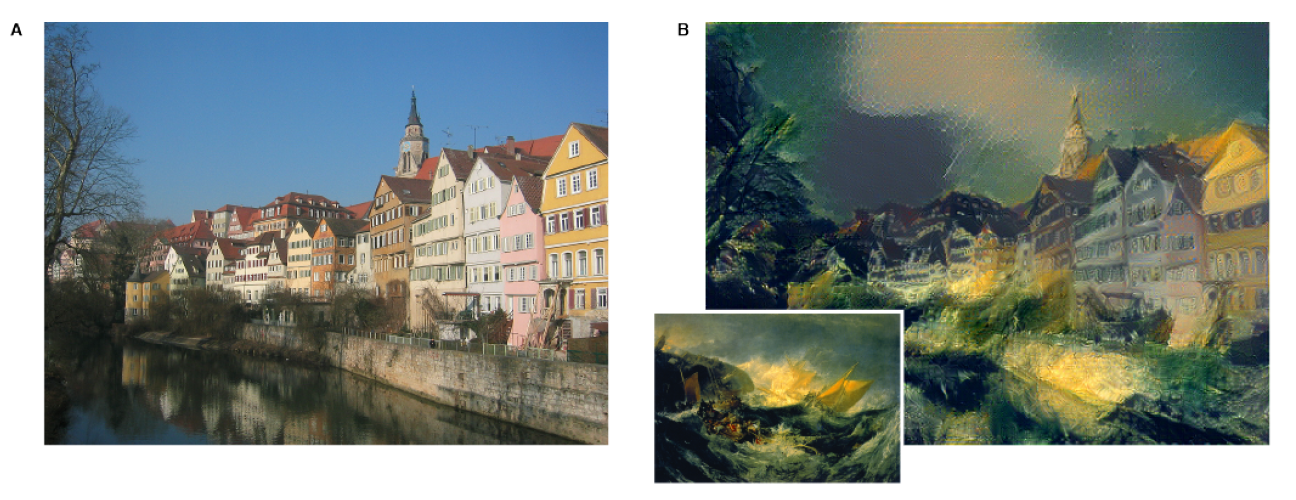
\includegraphics[width=\textwidth]{styletransfer}
        \caption{\label{fig:styletransfer}From: Gatys, 2015}
    \end{figure}

    \end{frame}

    \subsection{Introduction}

    \begin{frame}{Method of Johnson, 2016}

    \begin{itemize}
        \item Two networks:
            \begin{itemize}
                \item Image transform network (Deconv Net)
                \item Loss network (VGG Net)
            \end{itemize}
        \item Two losses: content loss + style loss
    \end{itemize}

    \begin{figure}
        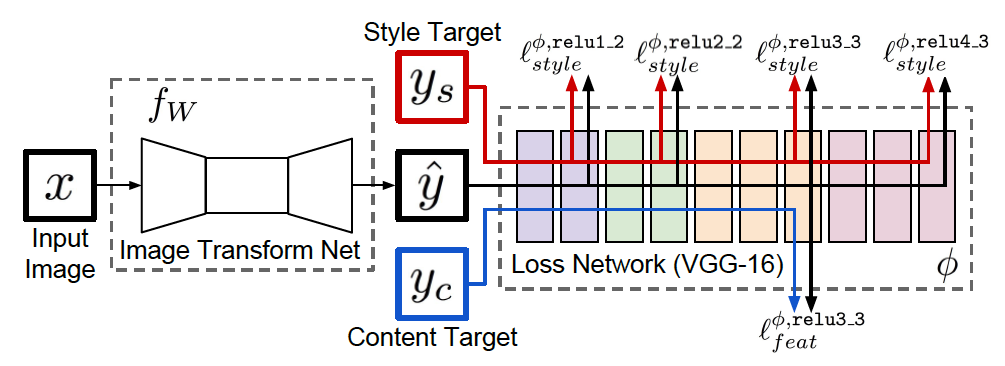
\includegraphics[width=\textwidth]{arch}
        \caption{\label{fig:arch}From: Johnson, 2016}
    \end{figure}

    \end{frame}

    \section{Lesson Learned}

    \begin{frame}{Lesson Learned}

    \begin{itemize}
        \item 20,000 training images is enough. Full epoch (~160k imgs) for COCO2014 needs ~3 hours of training!
        \item No free lunch: no hyperparams work for all styles. Also more on this later.
        \item Always use InstanceNorm instead of BatchNorm. More on this later.
        \item All of these images hencefort will use InstanceNorm unless specified.
    \end{itemize}

    \end{frame}

    \section{Experiments}

    \subsection{Styles used}

    \begin{frame}{Style images}

        \begin{figure}
            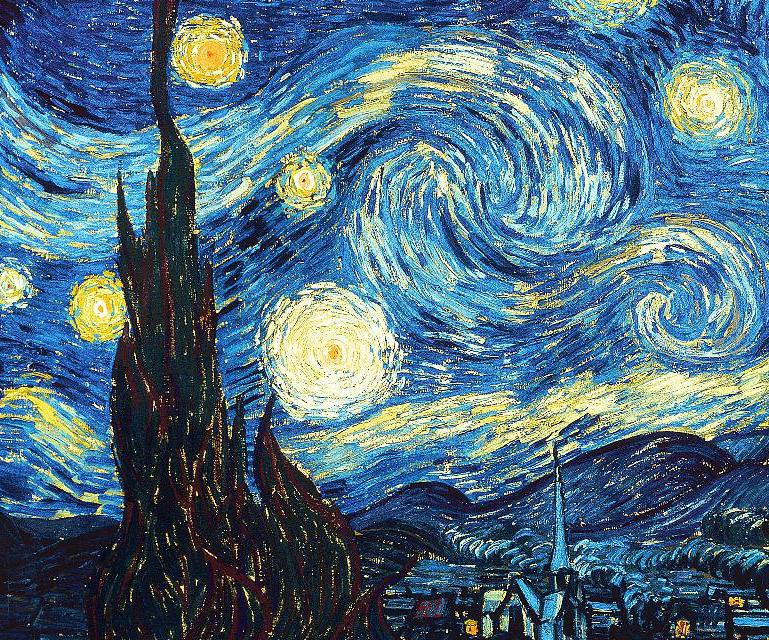
\includegraphics[width=0.495\textwidth]{starry}
            \hfill
            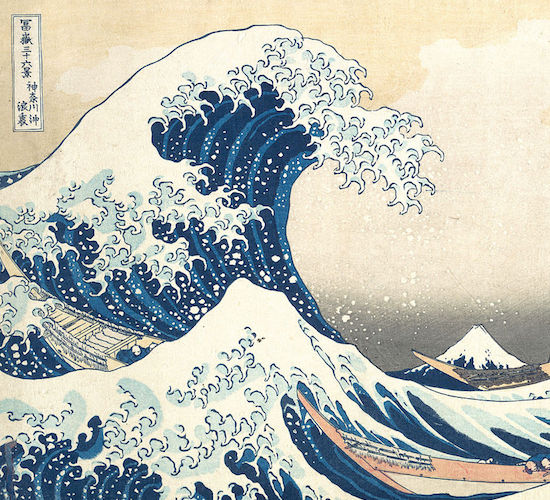
\includegraphics[width=0.495\textwidth]{tsunami}
            \caption{\label{fig:style_paper}Style images as in Johnson 2016}
        \end{figure}

    \end{frame}

    \begin{frame}{Style images}

        \begin{figure}
            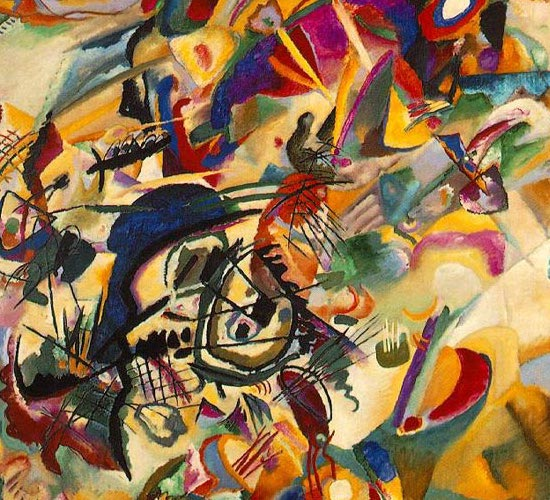
\includegraphics[width=0.32\textwidth]{compo}
            \hfill
            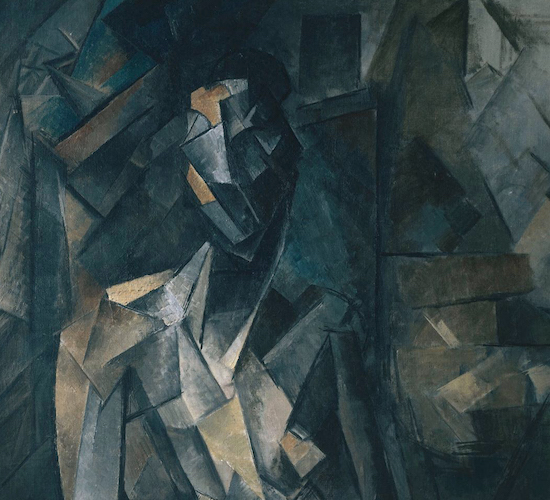
\includegraphics[width=0.32\textwidth]{femme}
            \hfill
            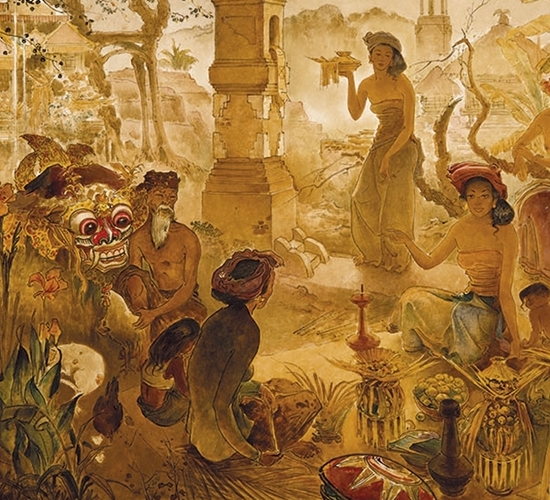
\includegraphics[width=0.32\textwidth]{bali}
            \caption{\label{fig:noisy}Our own style images}
        \end{figure}

    \end{frame}

    \subsection{Results}

    \begin{frame}{Effect of noise}

        \begin{figure}
            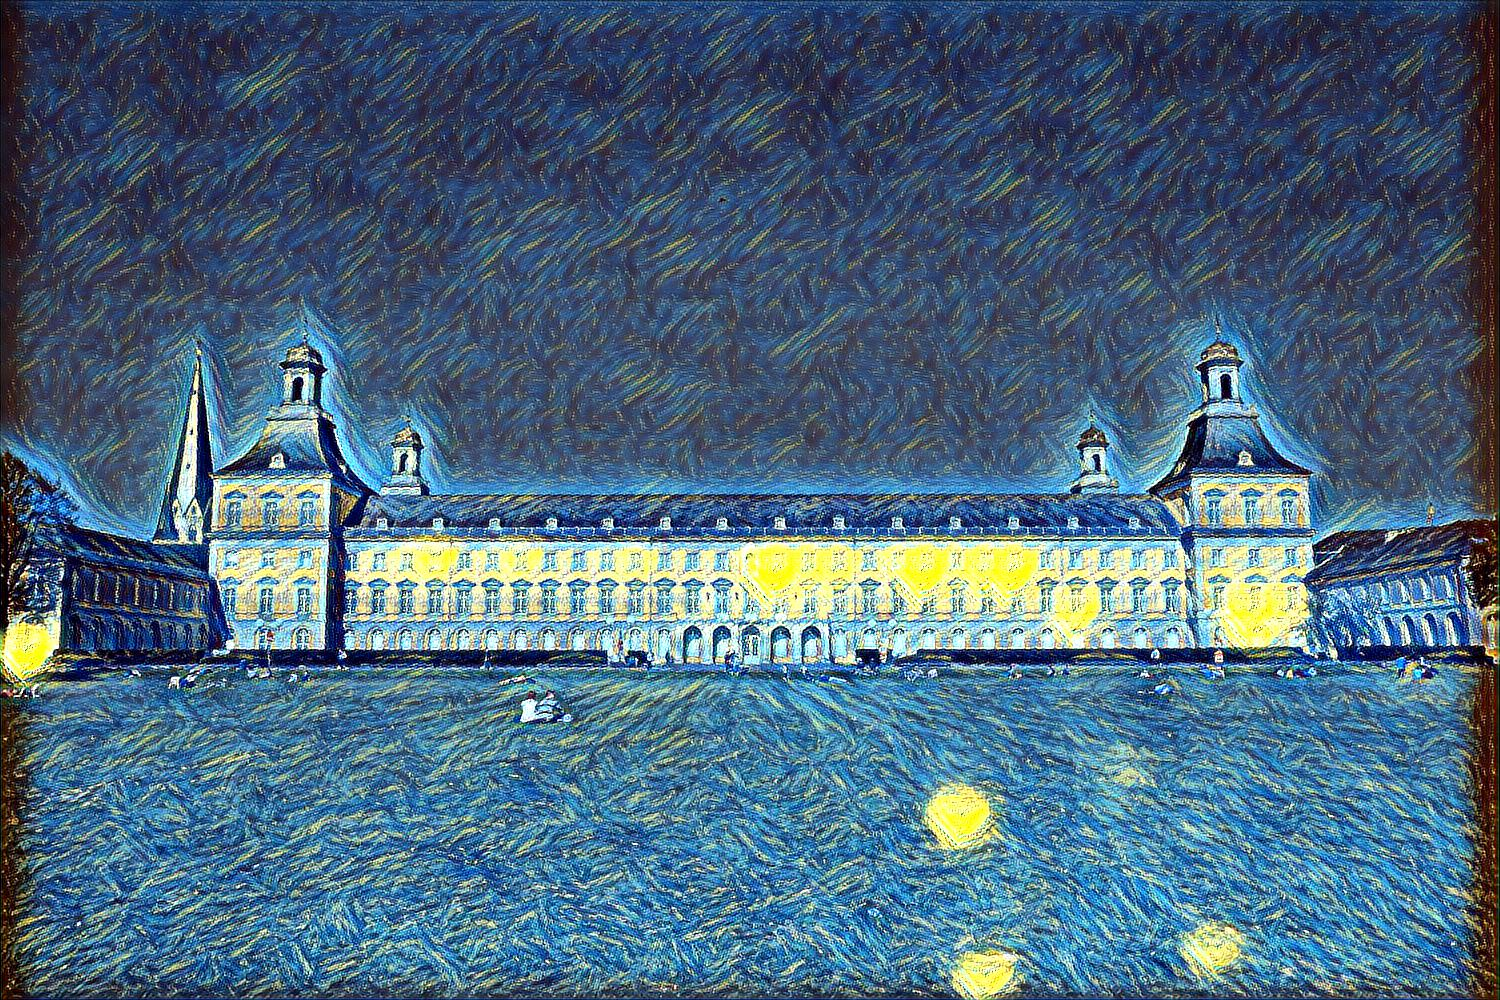
\includegraphics[width=0.495\textwidth]{clean}
            \hfill
            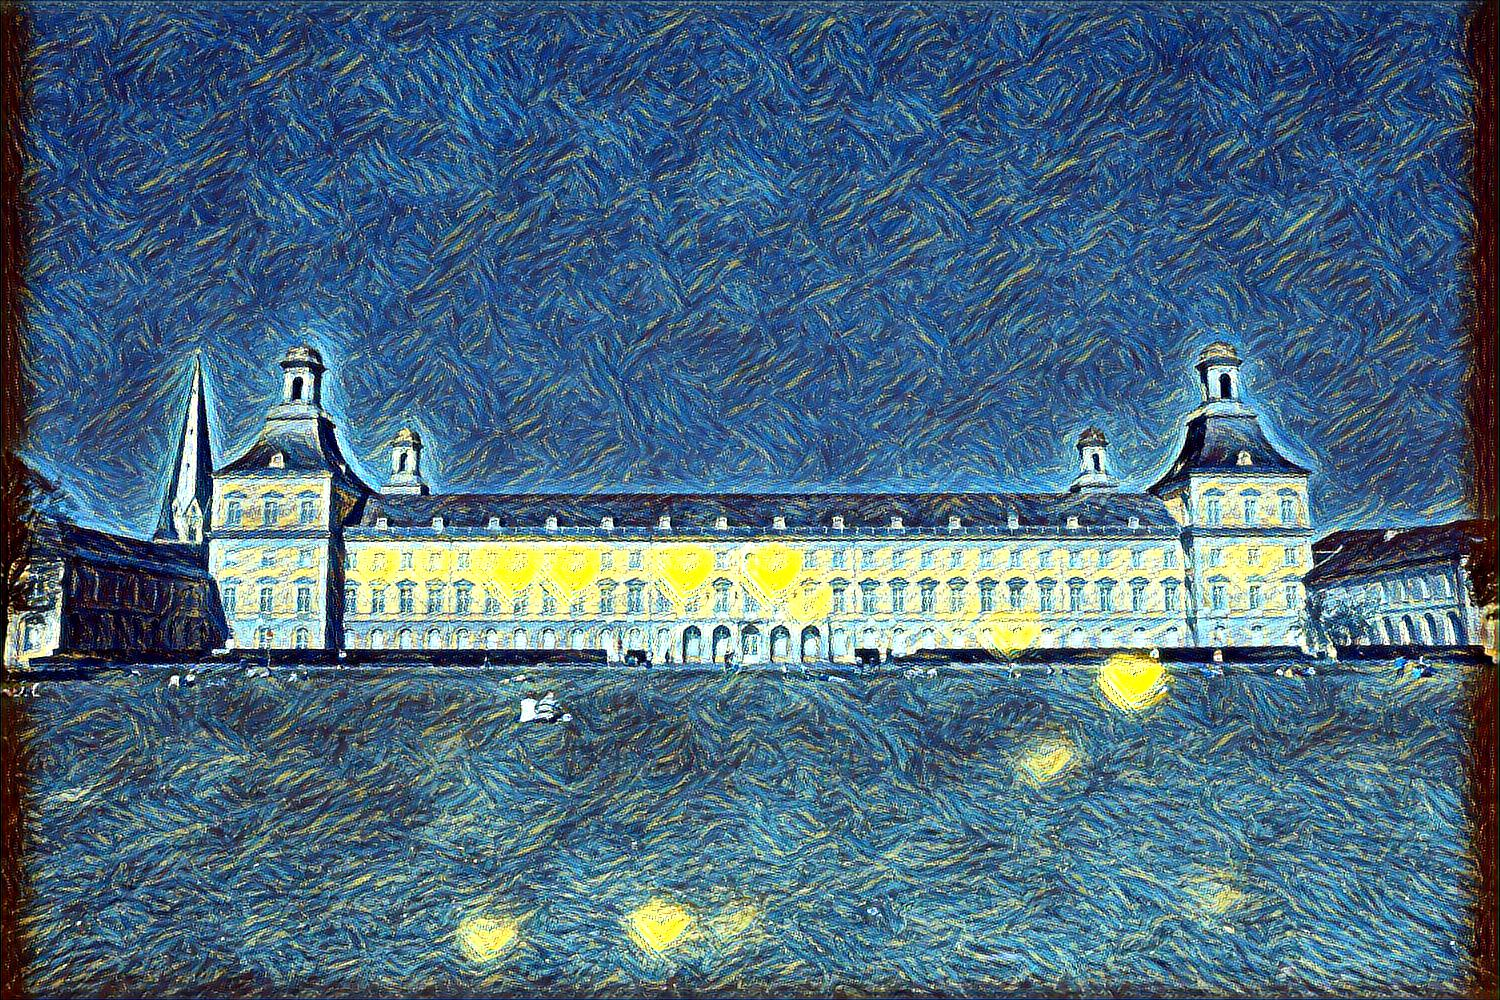
\includegraphics[width=0.495\textwidth]{noisy}
            \caption{\label{fig:noisy}Starry Night: Clean vs Noisy}
        \end{figure}

    \end{frame}

    \begin{frame}{Effect of clutter}

        \begin{figure}
            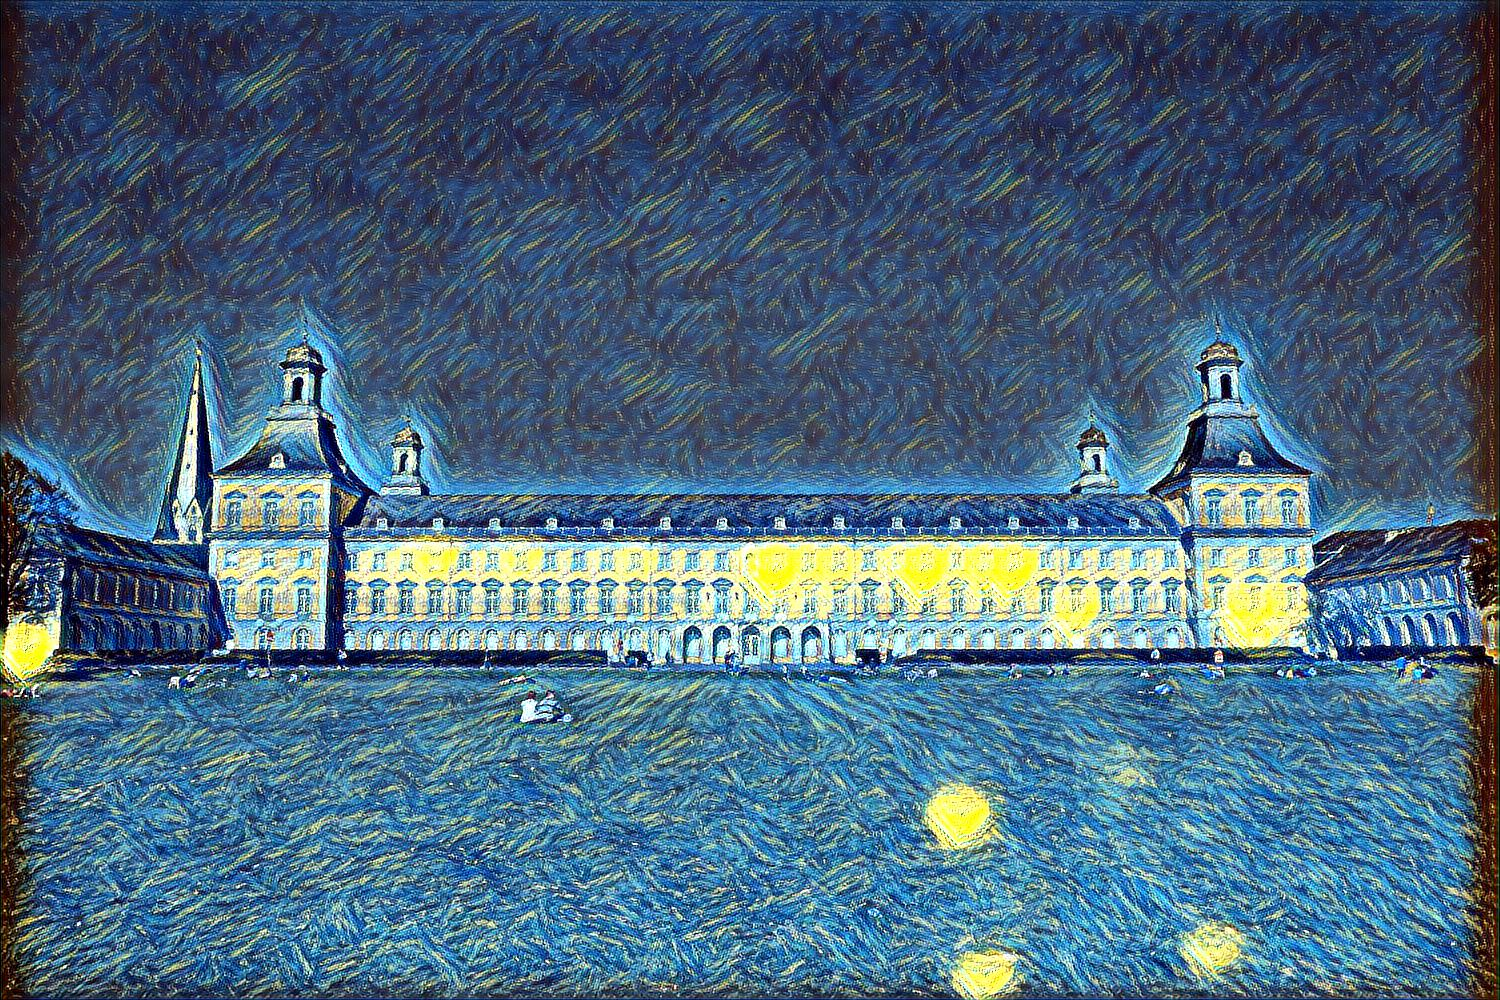
\includegraphics[width=0.495\textwidth]{clean}
            \hfill
            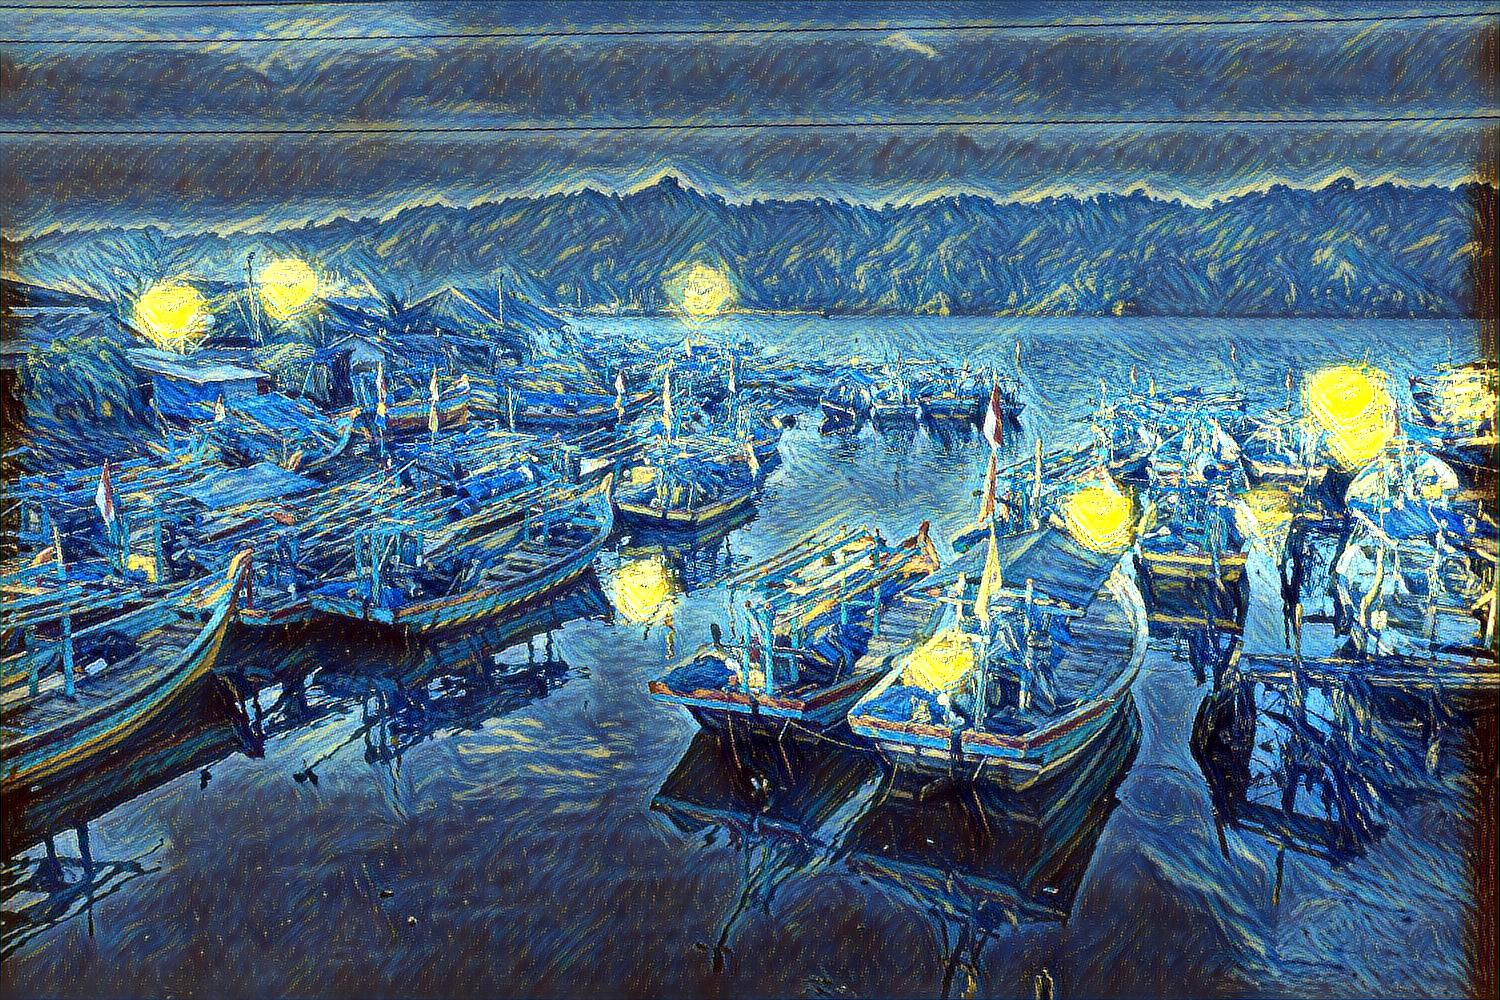
\includegraphics[width=0.495\textwidth]{clutter}
            \caption{\label{fig:clutter}Starry Night: Clean vs Clutter}
        \end{figure}

    \end{frame}

    \begin{frame}{Outdoor vs indoor}

        \begin{figure}
            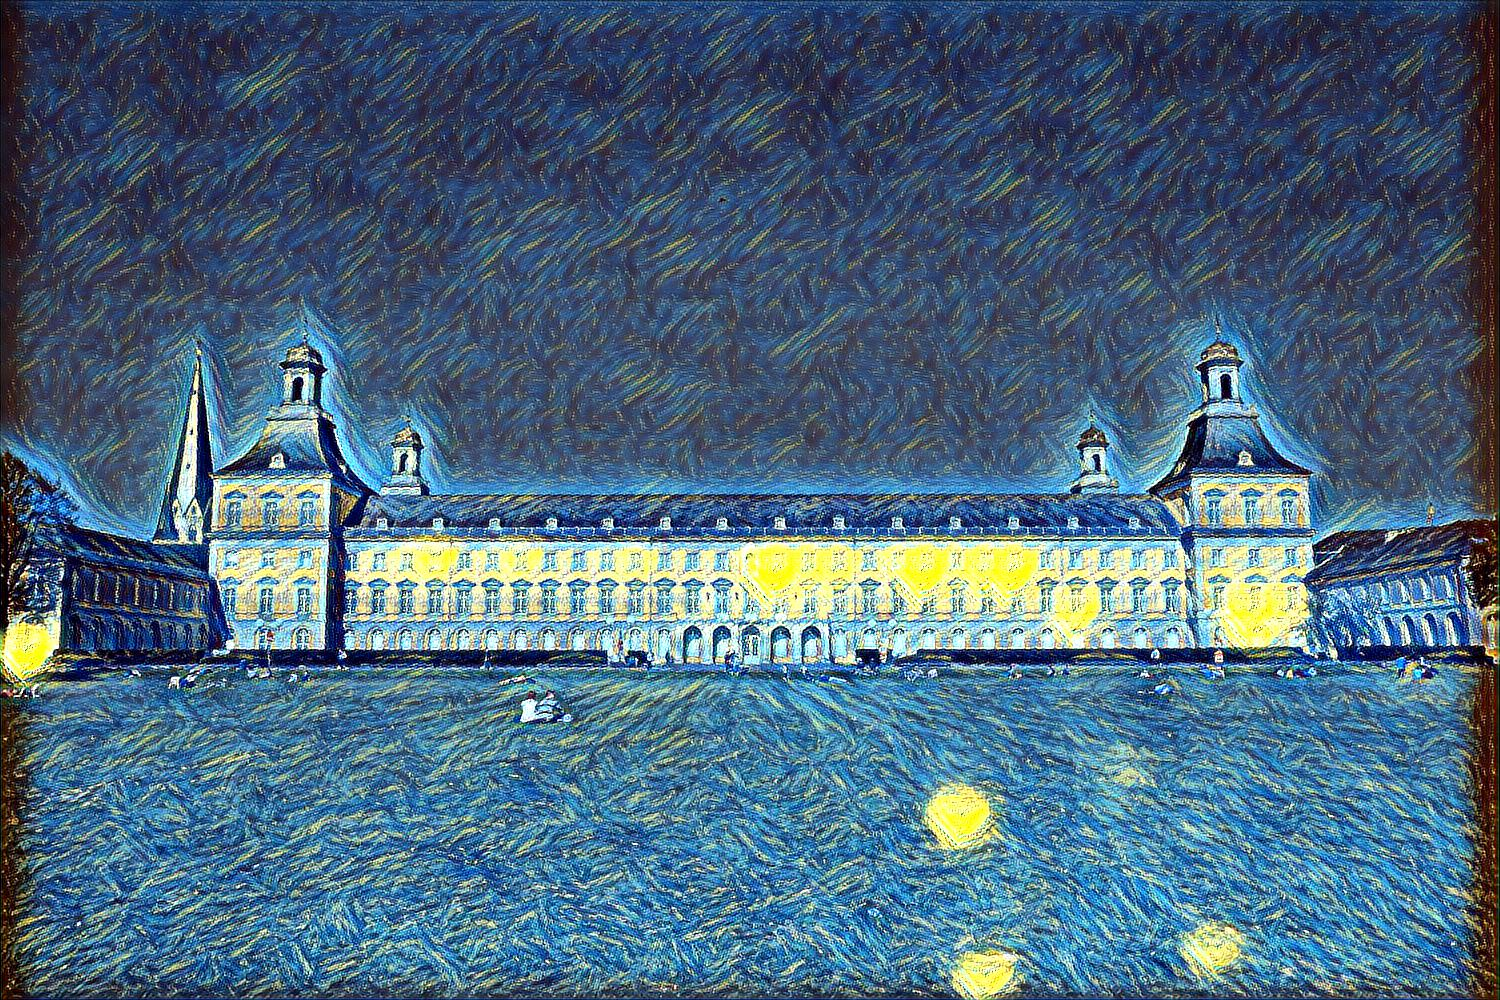
\includegraphics[width=0.495\textwidth]{clean}
            \hfill
            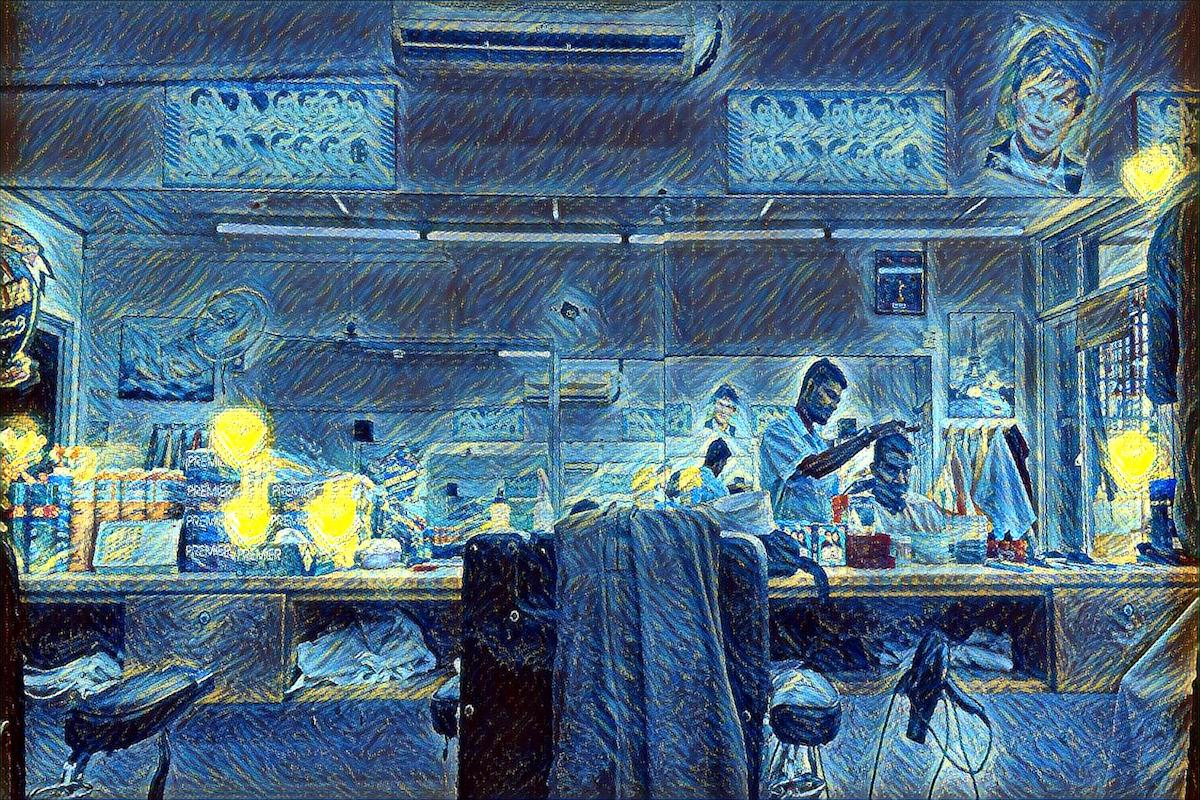
\includegraphics[width=0.495\textwidth]{indoor}
            \caption{\label{fig:clutter}Starry Night: Outdoor vs Indoor}
        \end{figure}

    \end{frame}

    \begin{frame}{Effect of image size}

        \begin{figure}
            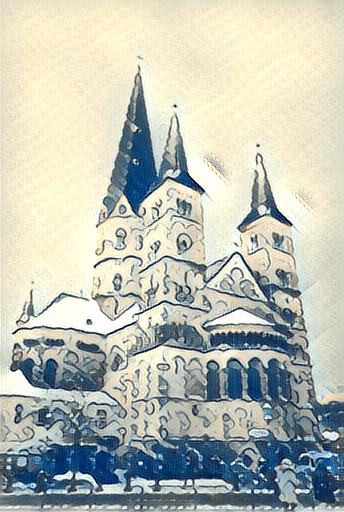
\includegraphics[width=0.495\textwidth, height=0.7\textheight]{small}
            \hfill
            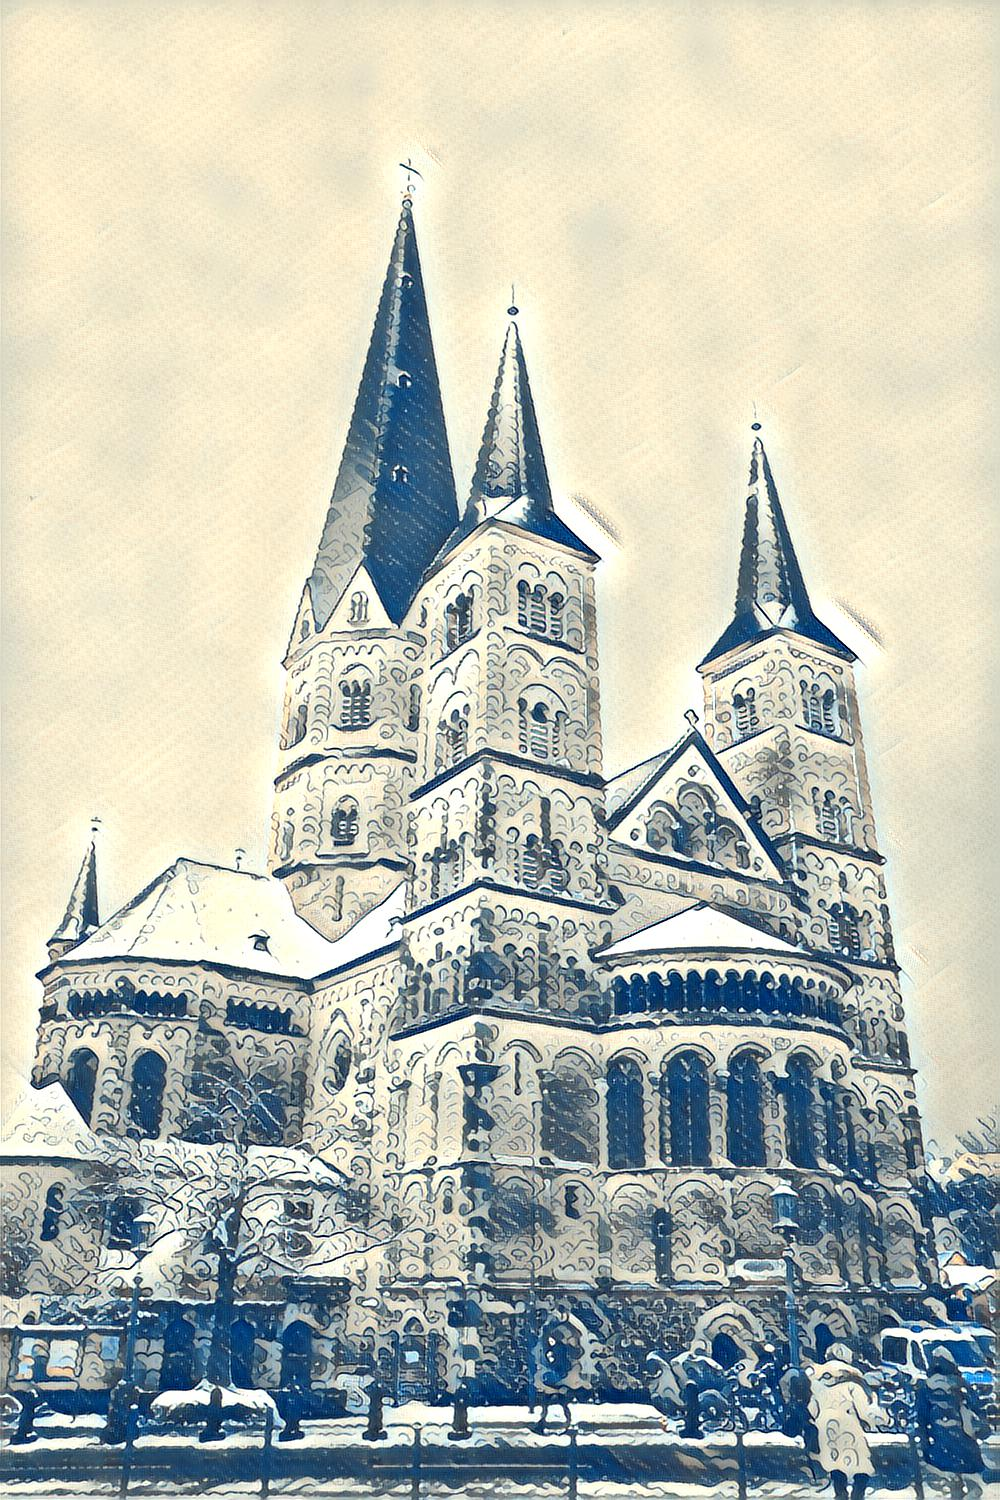
\includegraphics[width=0.495\textwidth, height=0.7\textheight]{large}
            \caption{\label{fig:clutter}Great Wave of Kanagawa: Small vs Large}
        \end{figure}

    \end{frame}

    \begin{frame}{New styles}

        \begin{figure}
            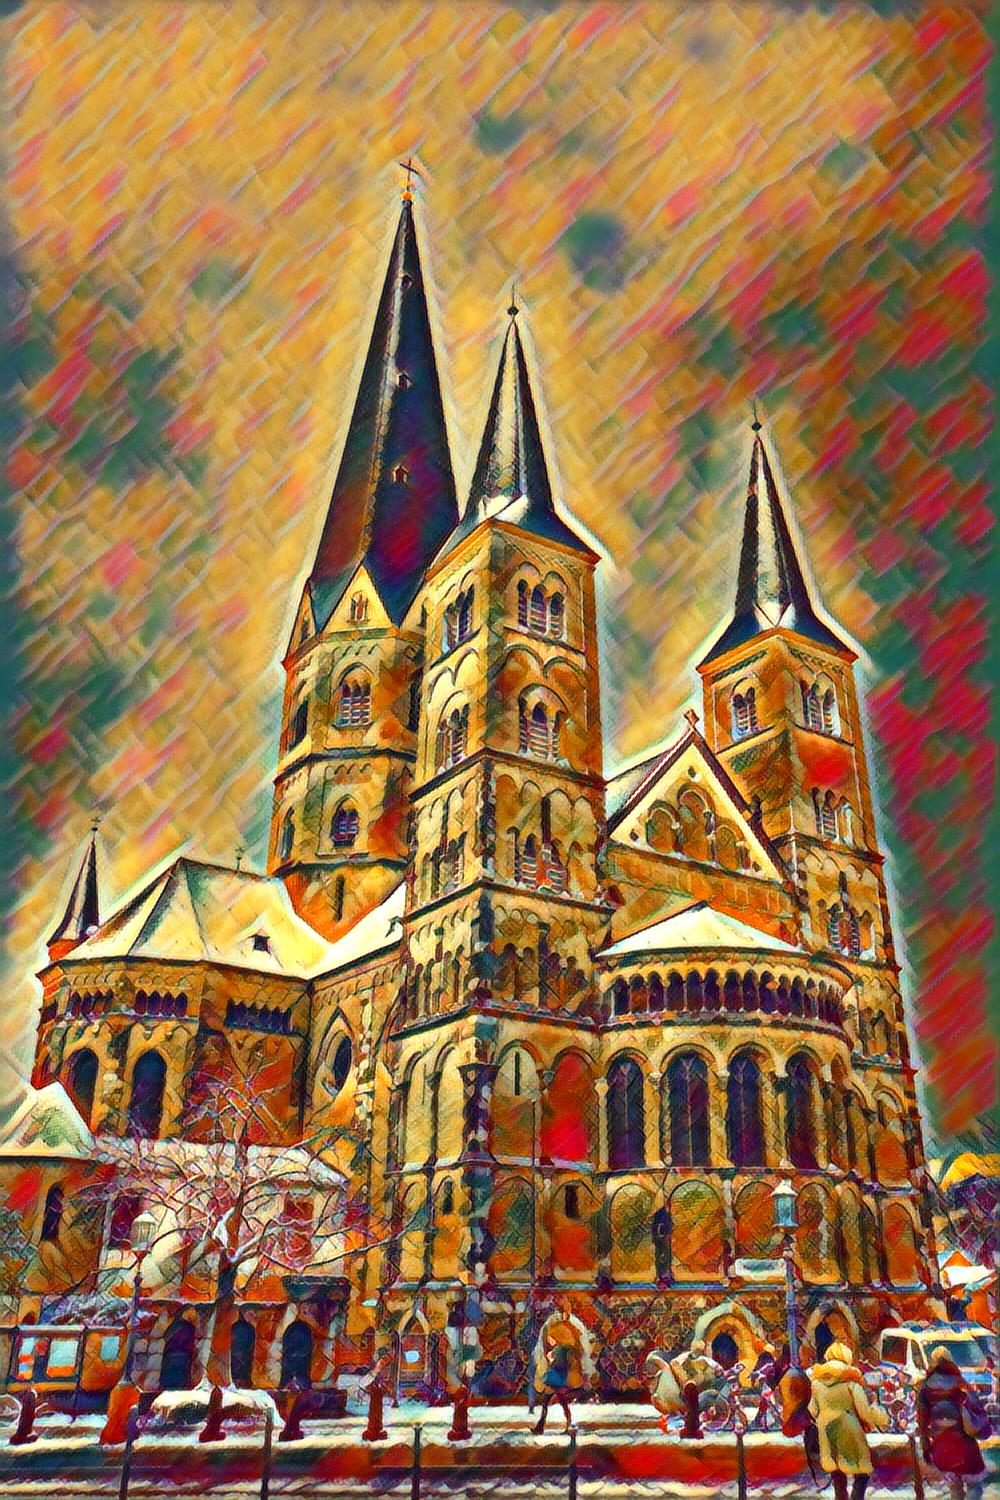
\includegraphics[width=0.325\textwidth, height=0.6\textheight]{mu_compo}
            \hfill
            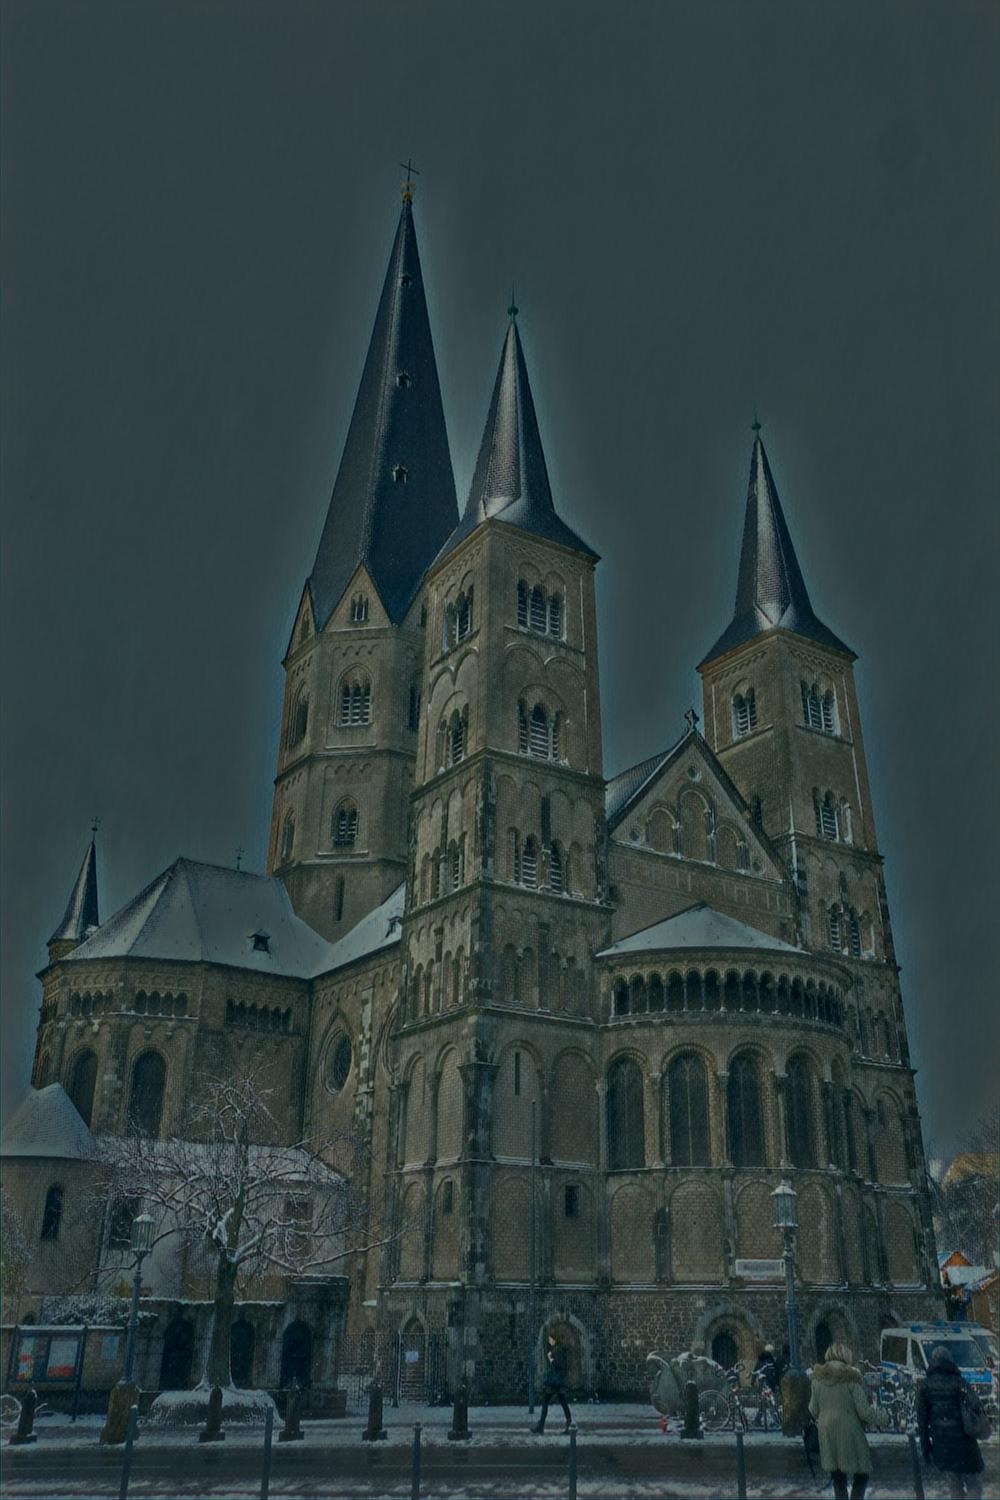
\includegraphics[width=0.325\textwidth, height=0.6\textheight]{mu_femme}
            \hfill
            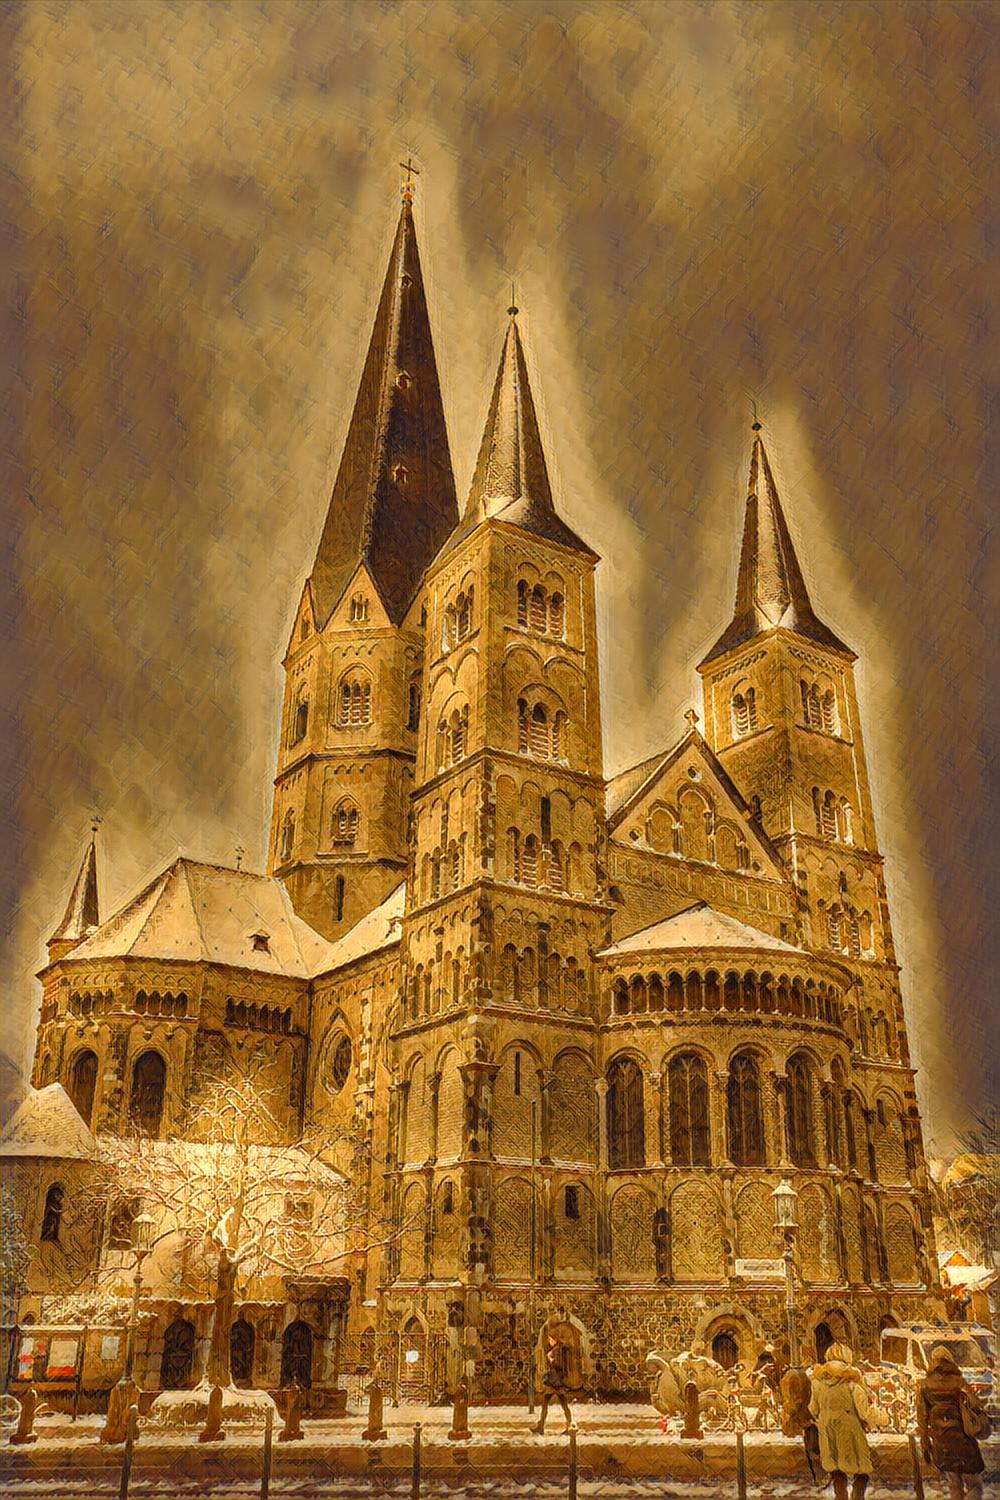
\includegraphics[width=0.325\textwidth, height=0.6\textheight]{mu_bali}
            \caption{\label{fig:clutter}New styles}
        \end{figure}

    \end{frame}

    \begin{frame}{InstanceNorm vs BatchNorm}

        \begin{figure}
            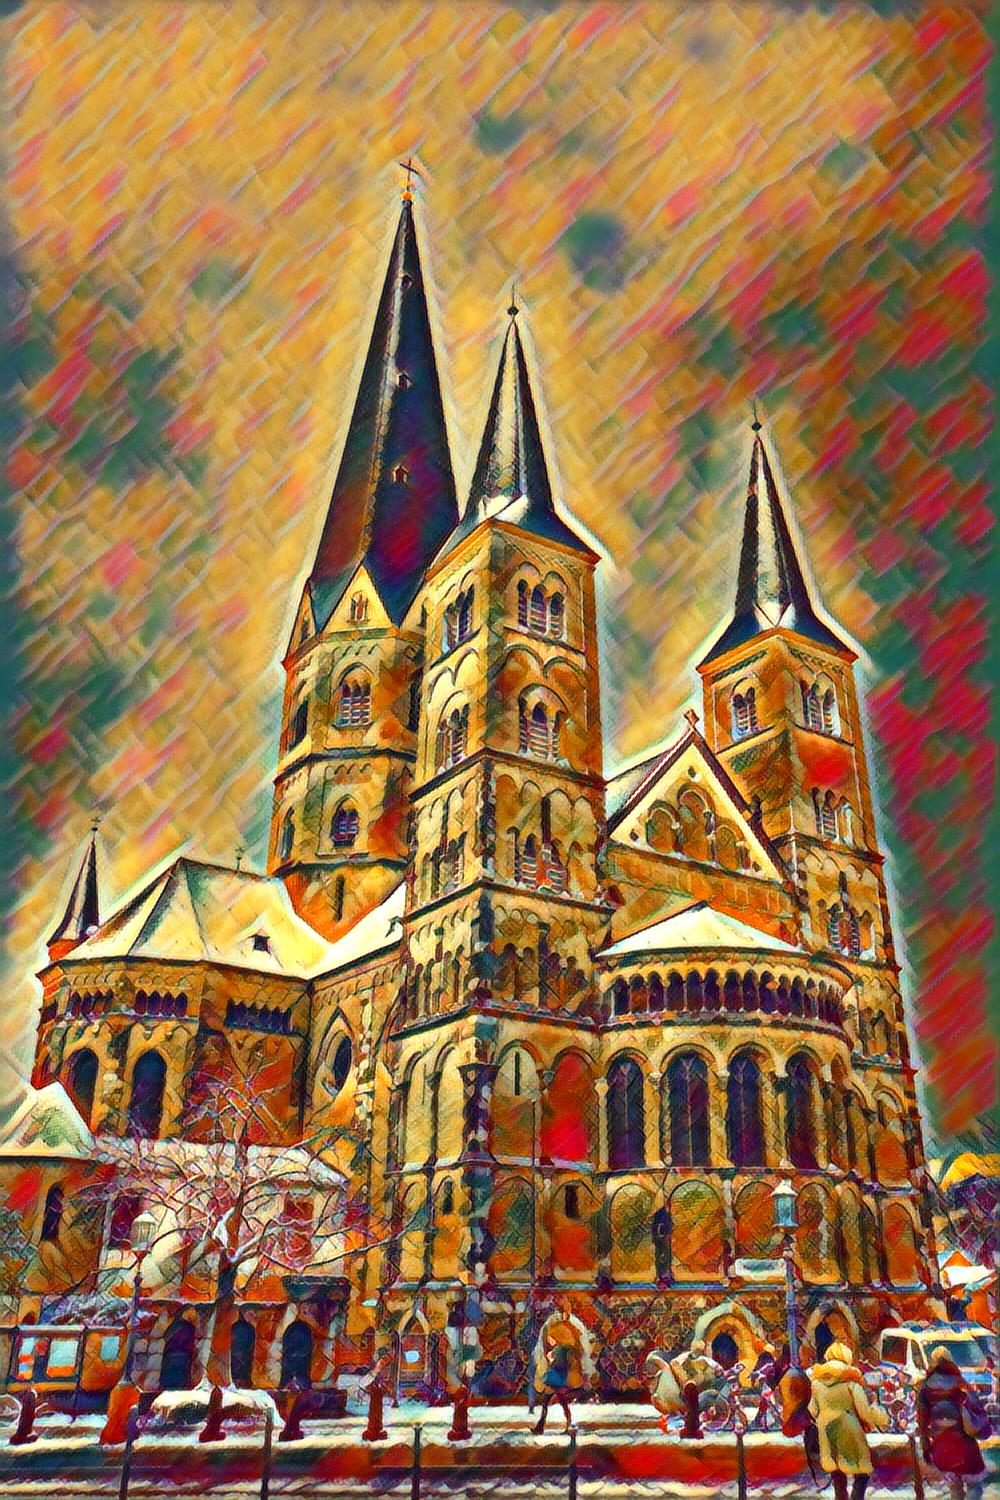
\includegraphics[width=0.495\textwidth, height=0.7\textheight]{mu_compo}
            \hfill
            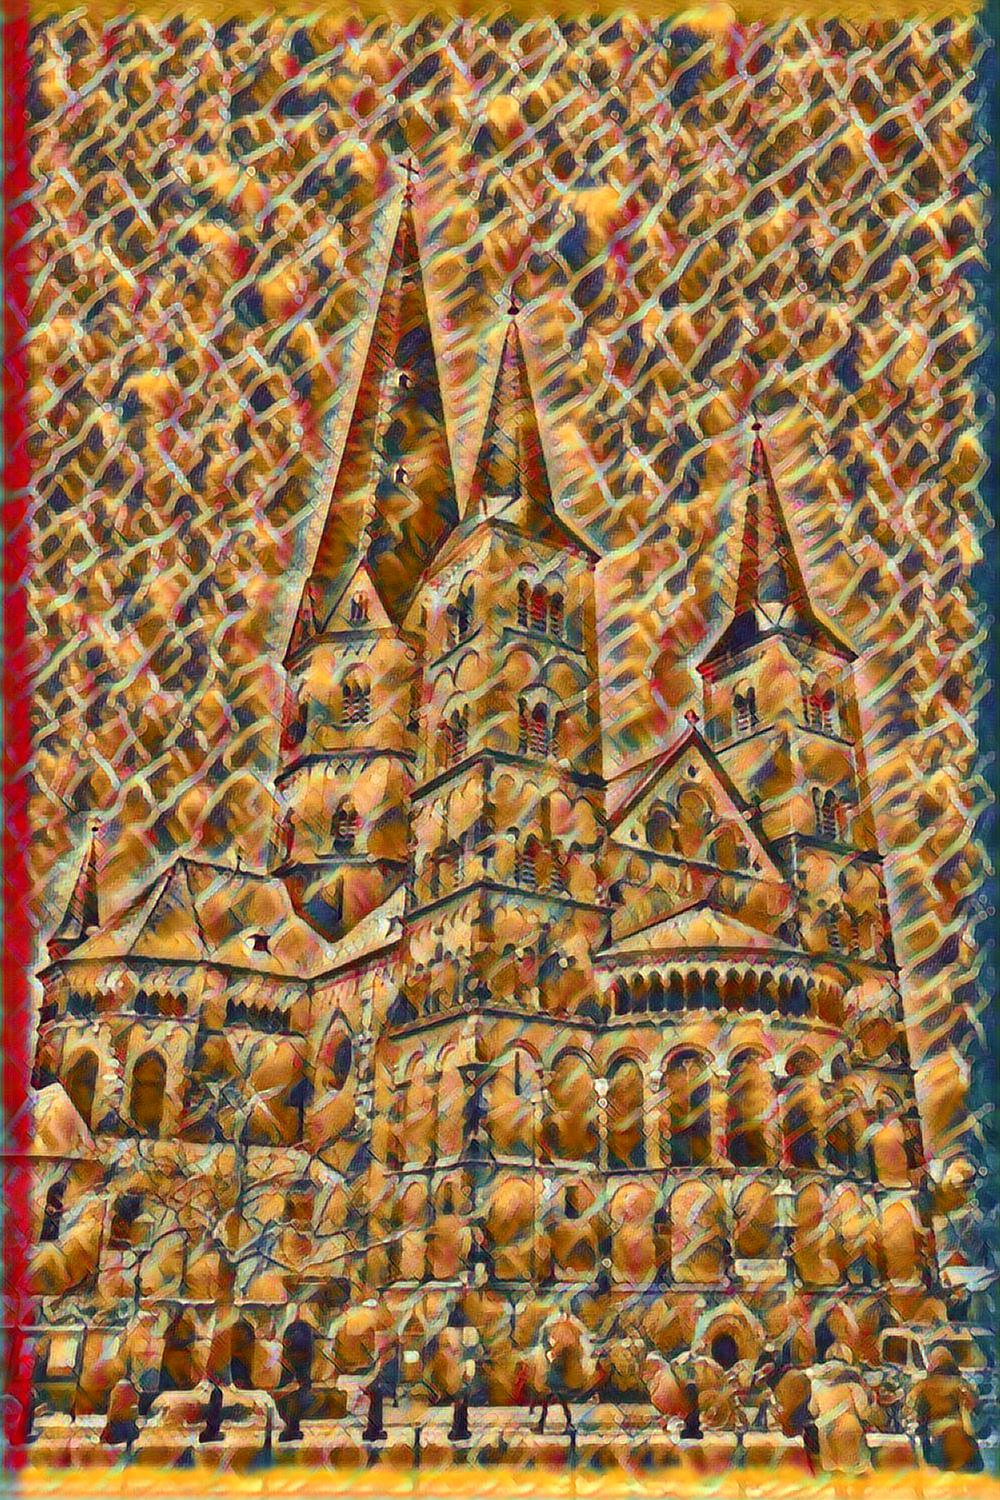
\includegraphics[width=0.495\textwidth, height=0.7\textheight]{mu_compo_bn}
            \caption{\label{fig:clutter}IN vs BN}
        \end{figure}

    \end{frame}

    \begin{frame}{Only one loss}

        \begin{figure}
            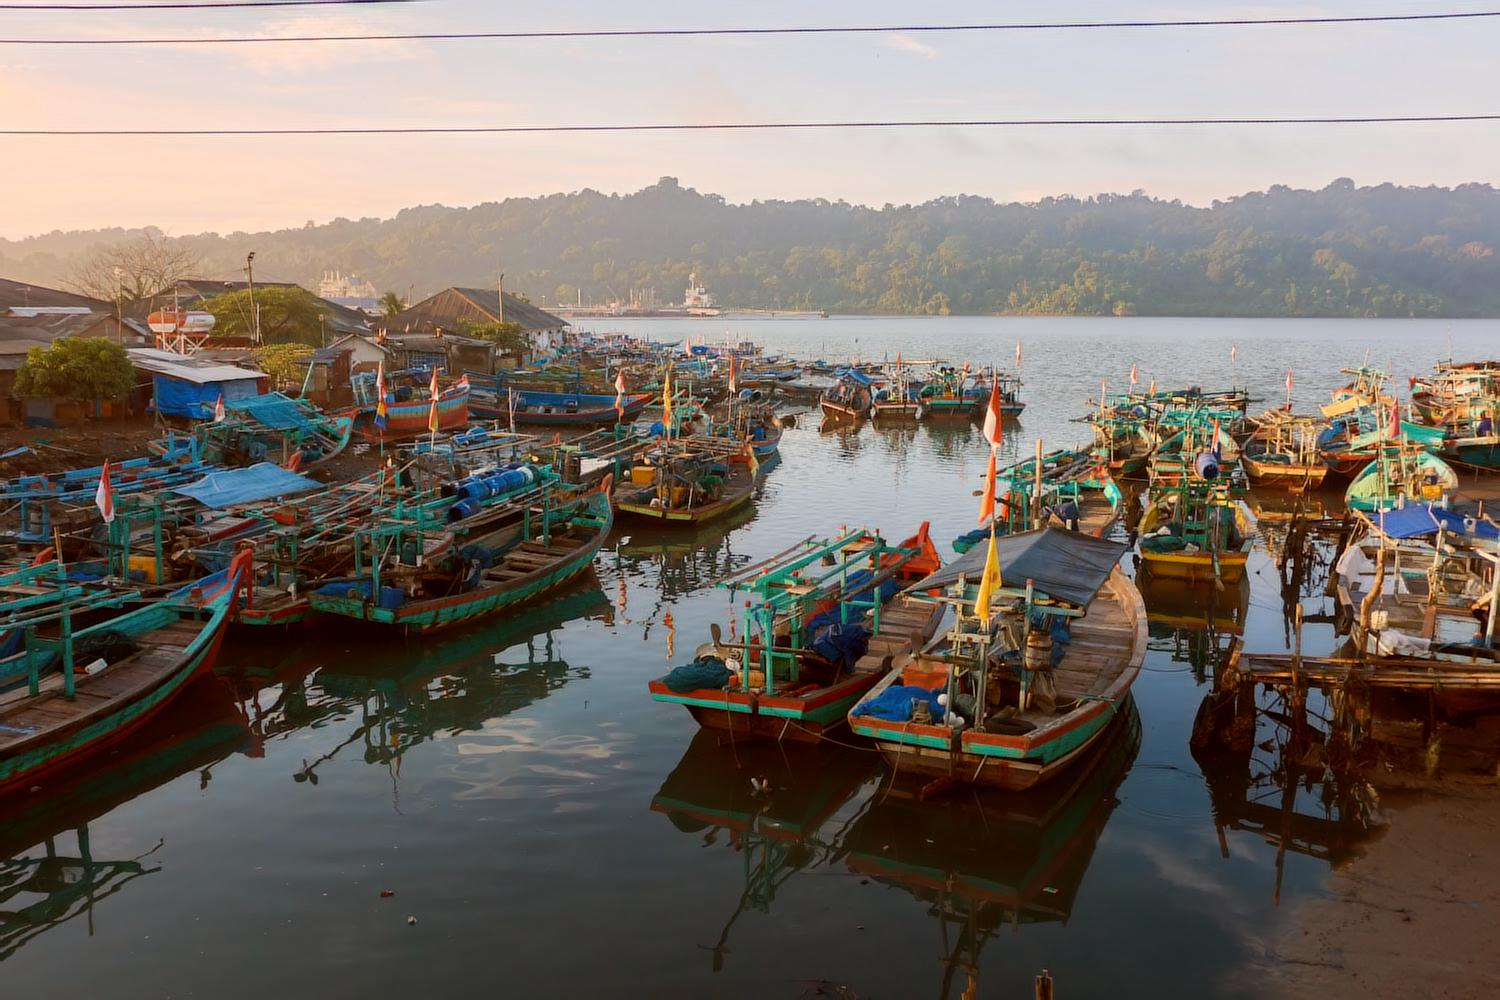
\includegraphics[width=0.495\textwidth]{nostyle}
            \hfill
            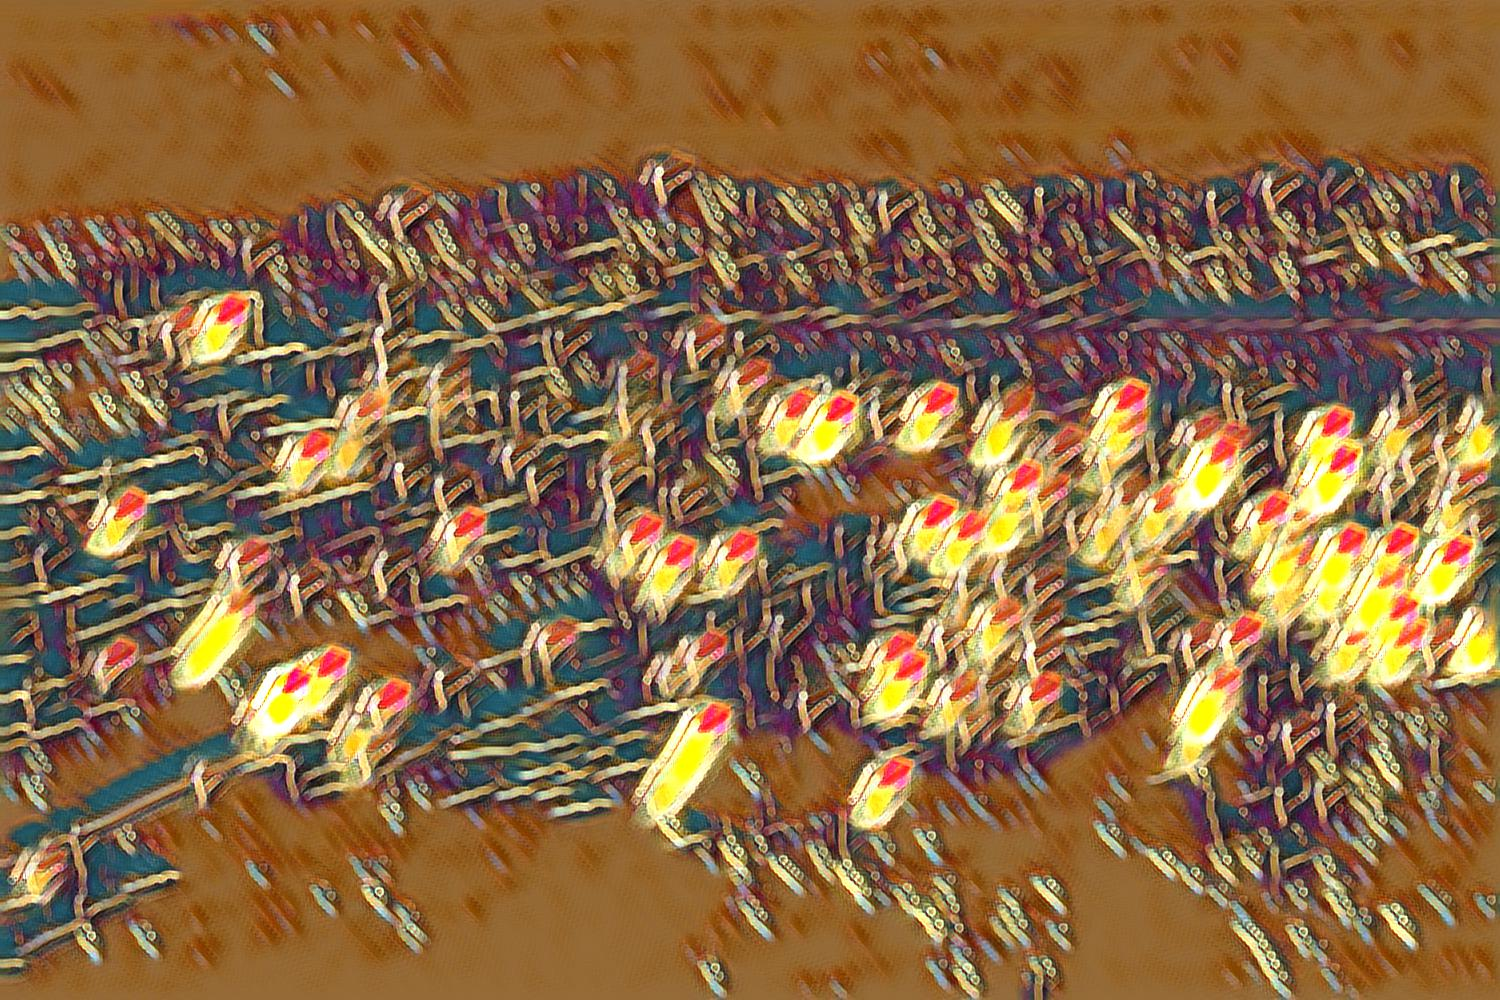
\includegraphics[width=0.495\textwidth]{nocontent}
            \caption{\label{fig:clutter}Only content vs only style}
        \end{figure}

    \end{frame}

    \begin{frame}{More style vs more content}

        \begin{figure}
            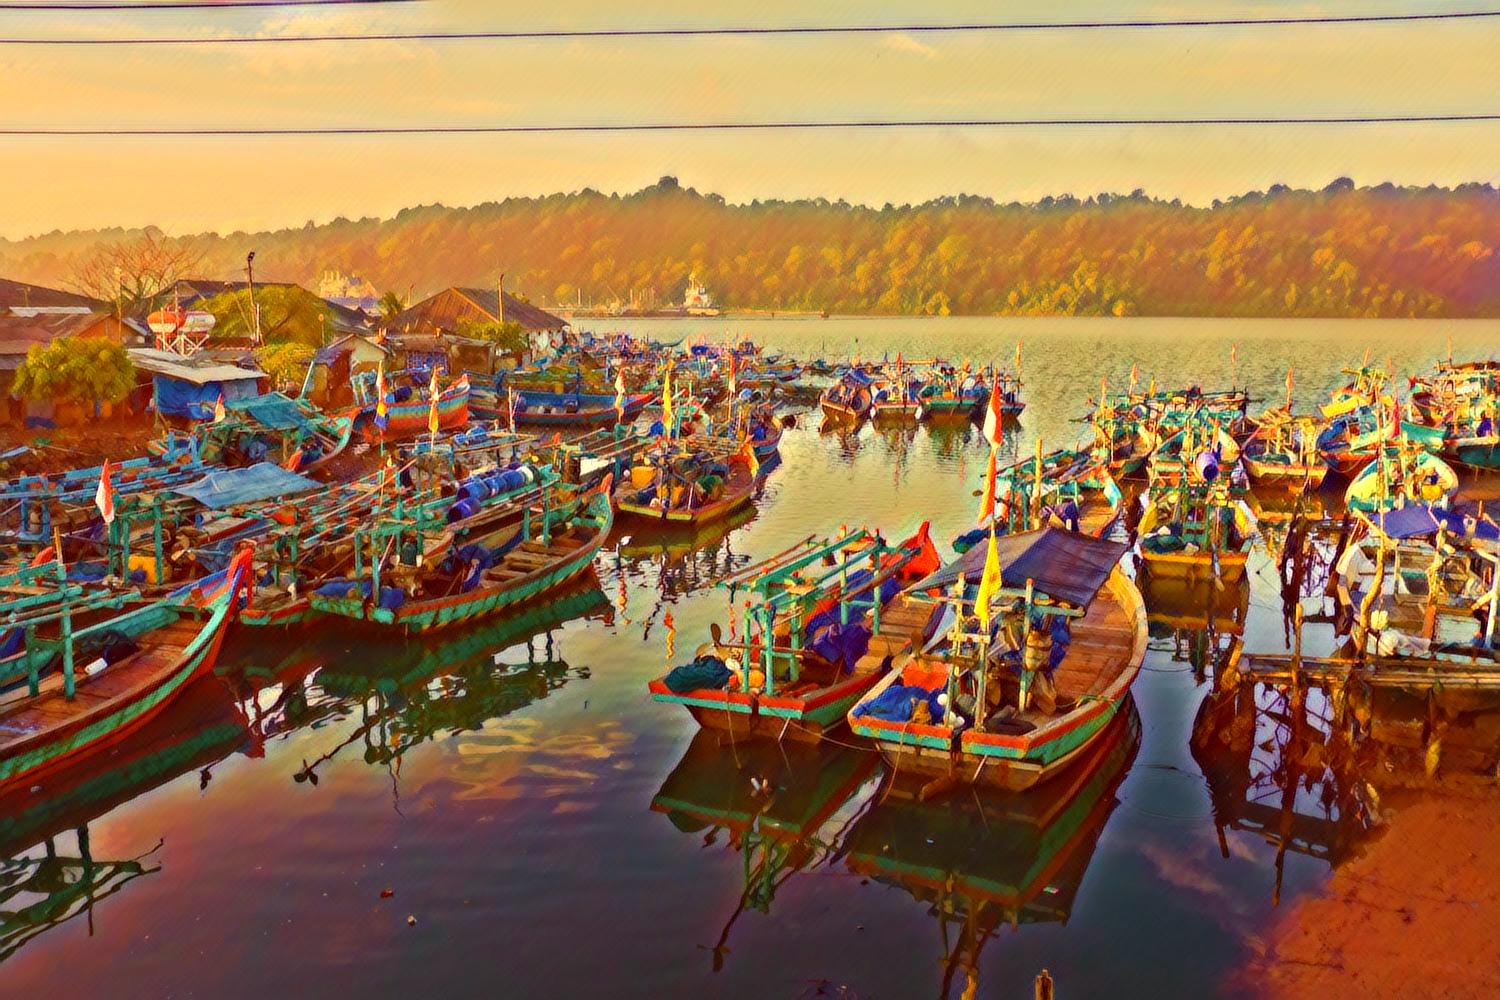
\includegraphics[width=0.495\textwidth]{morecontent}
            \hfill
            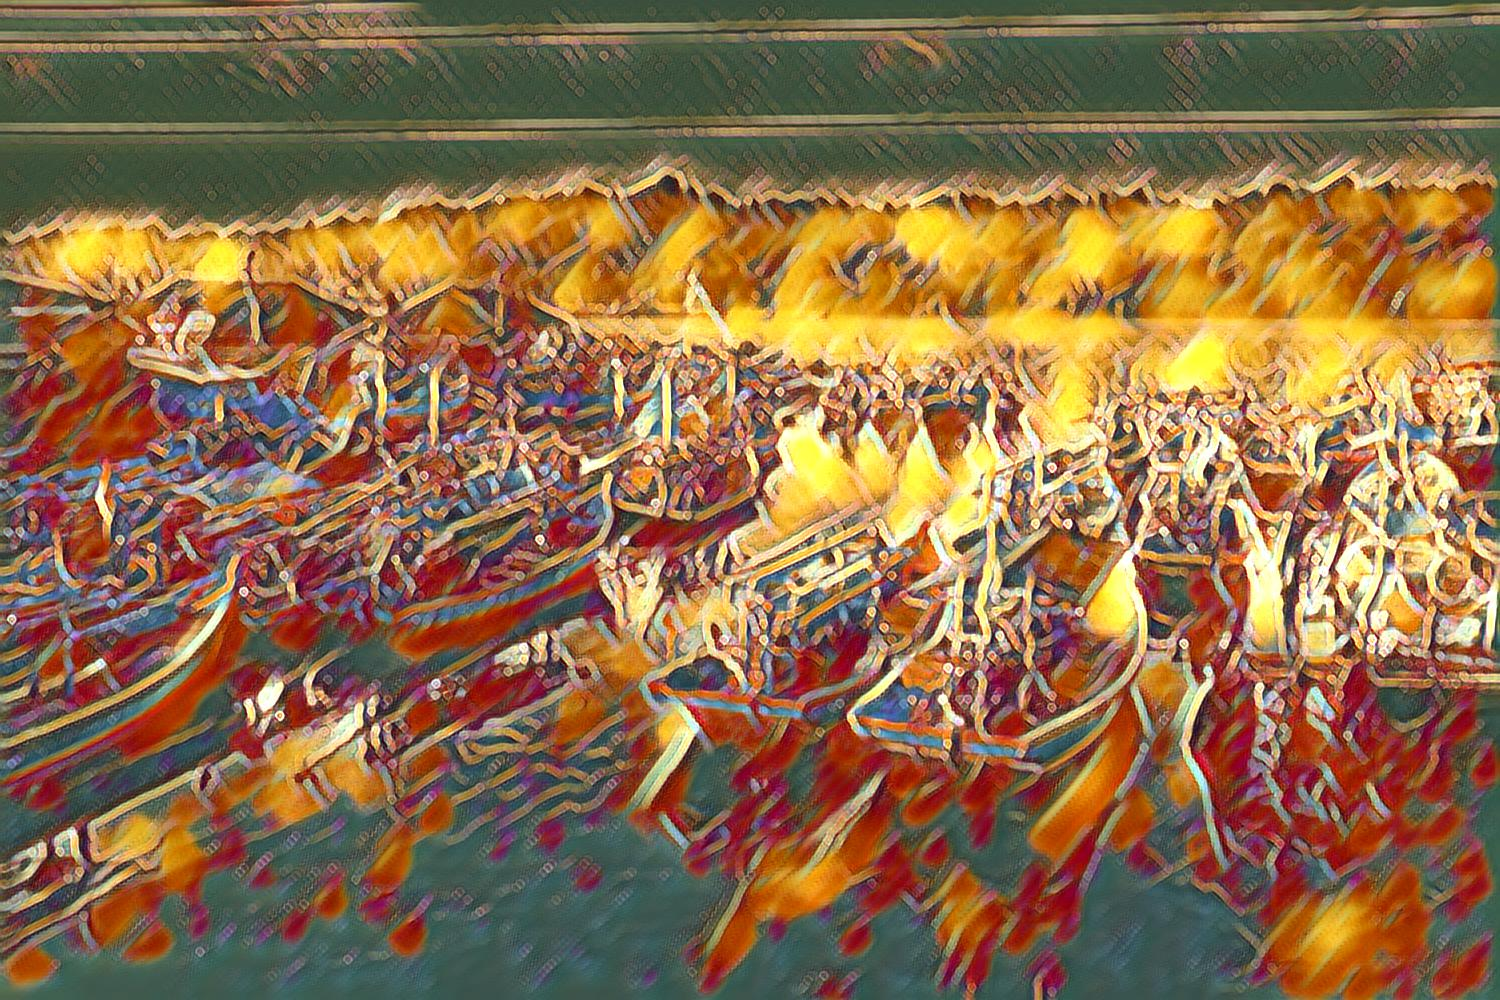
\includegraphics[width=0.495\textwidth]{morestyle}
            \caption{\label{fig:clutter}More content vs more style}
        \end{figure}

    \end{frame}

    \begin{frame}{Content loss: effect of layer choice}

        \begin{figure}
            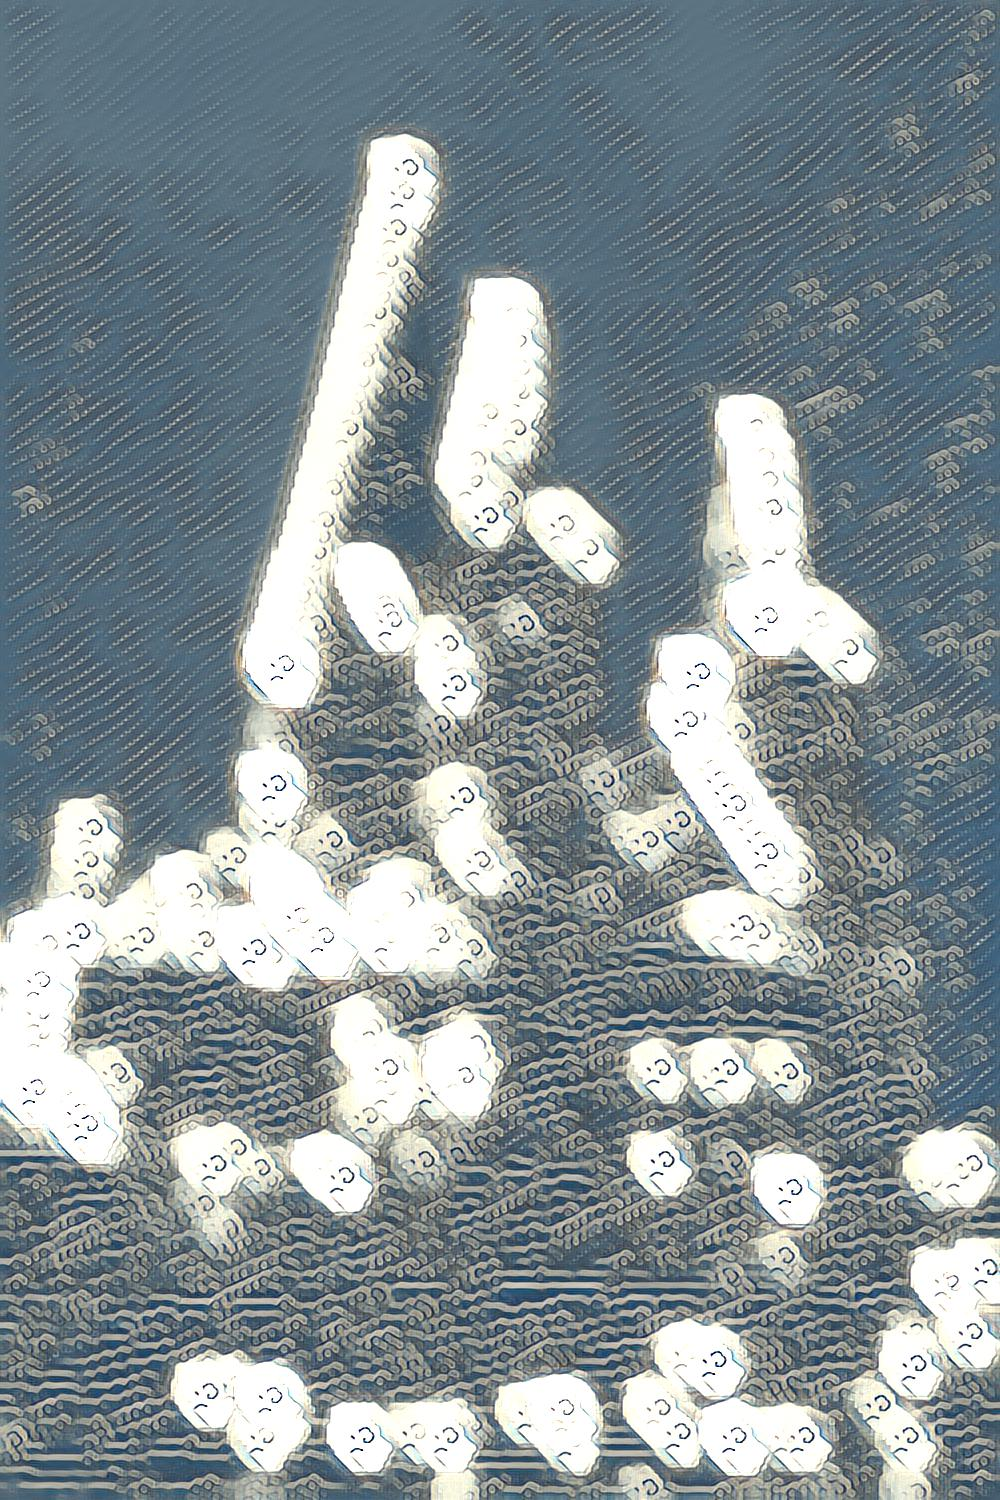
\includegraphics[width=0.248\textwidth, height=0.4\textheight]{bonn_muenster_tsunami_relu12}
            \hfill
            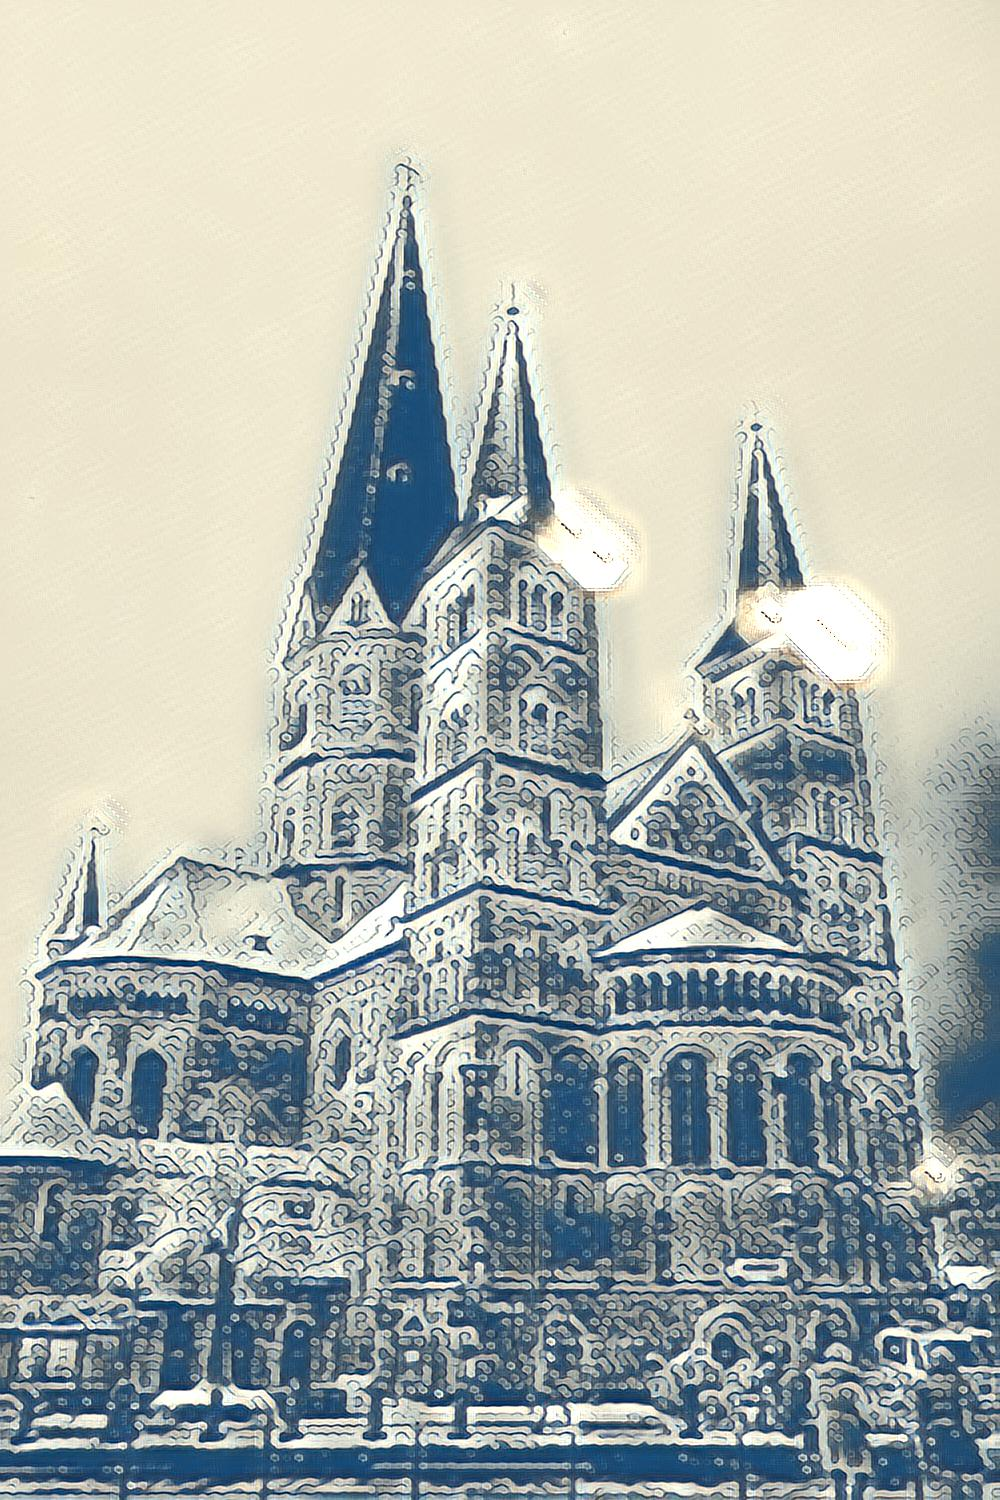
\includegraphics[width=0.248\textwidth, height=0.4\textheight]{bonn_muenster_tsunami_relu22}
            \hfill
            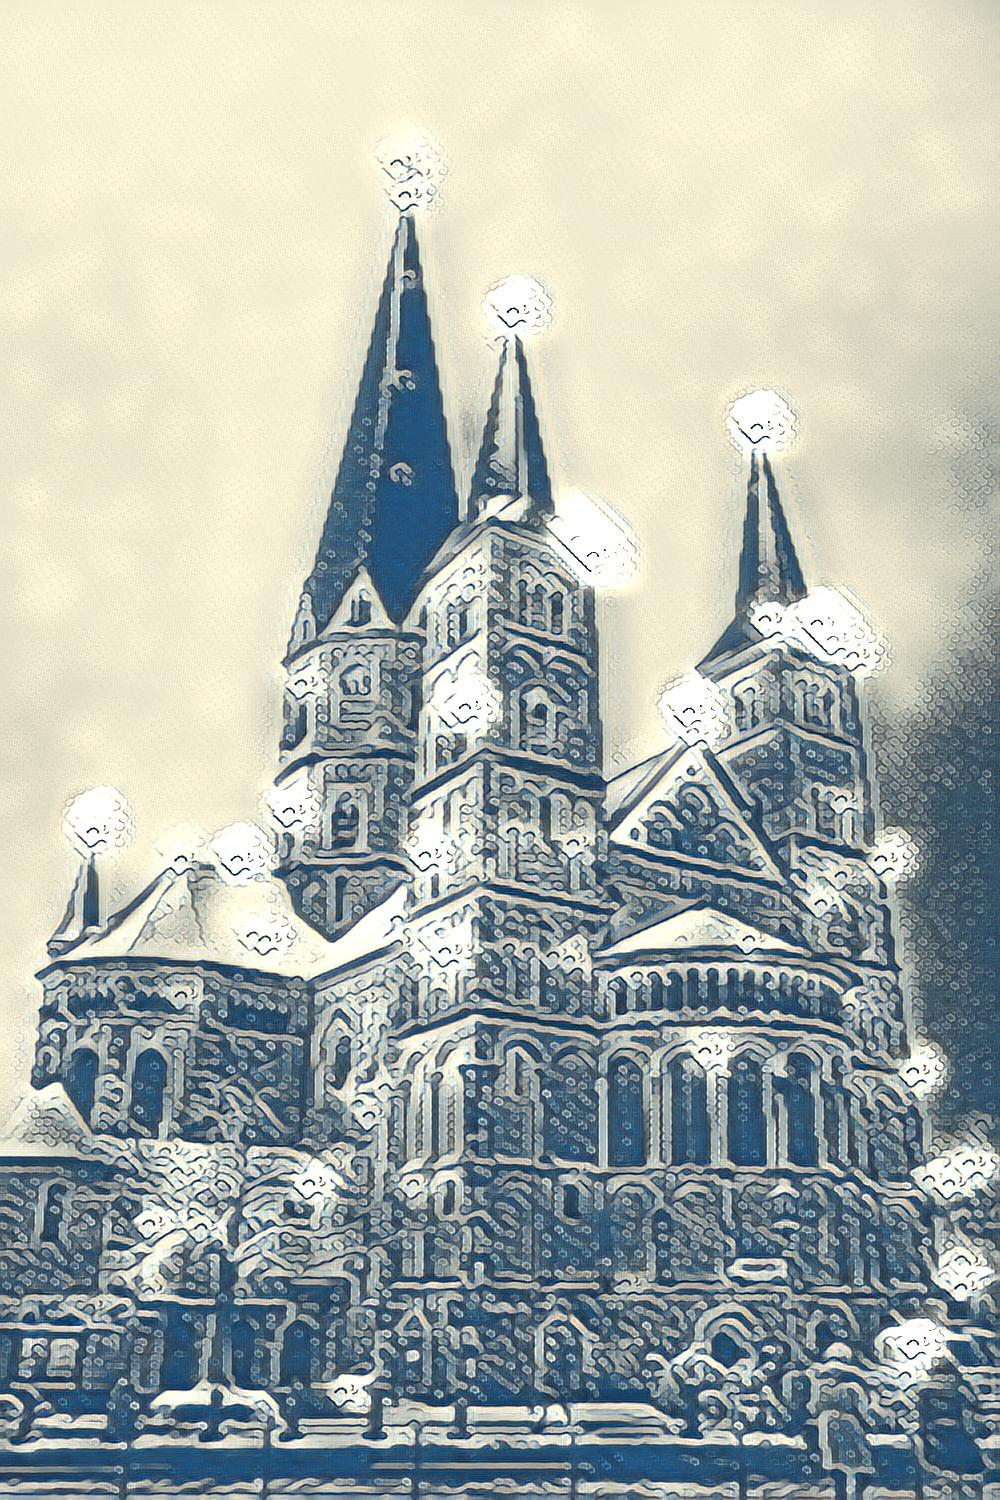
\includegraphics[width=0.248\textwidth, height=0.4\textheight]{bonn_muenster_tsunami_relu33}
            \hfill
            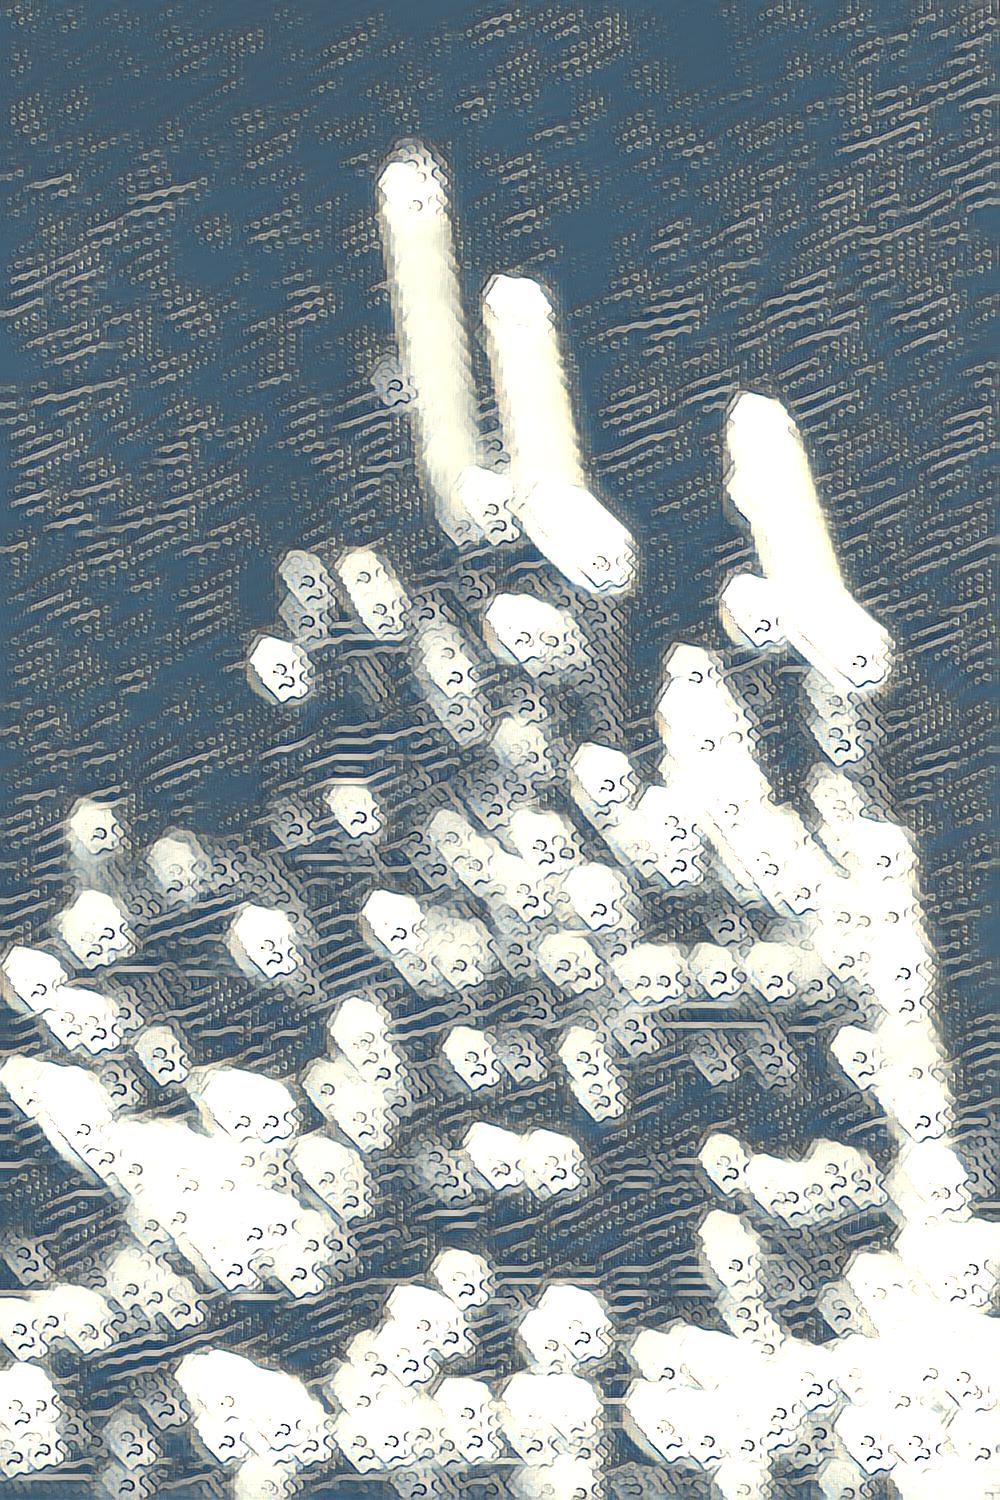
\includegraphics[width=0.248\textwidth, height=0.4\textheight]{bonn_muenster_tsunami_relu43}
            \caption{\label{fig:clutter}relu12 vs relu22 vs relu33 vs relu43}
        \end{figure}

    \end{frame}

    \begin{frame}{Style loss: effect of layers choice}

        \begin{figure}
            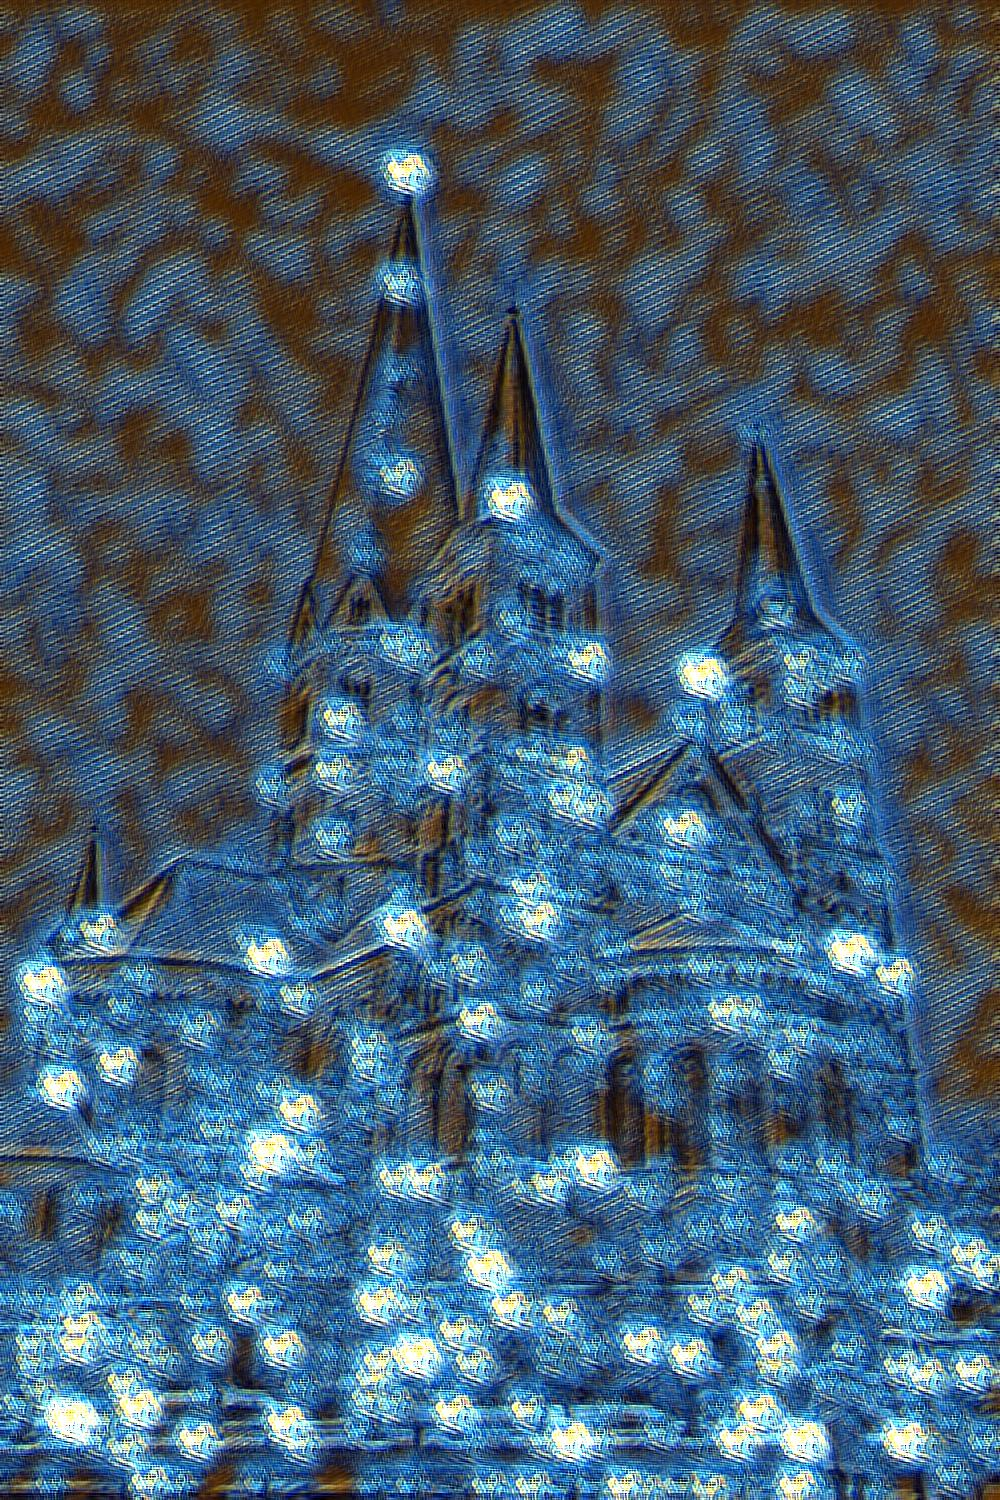
\includegraphics[width=0.495\textwidth, height=0.7\textheight]{bonn_muenster_starry_style_lower}
            \hfill
            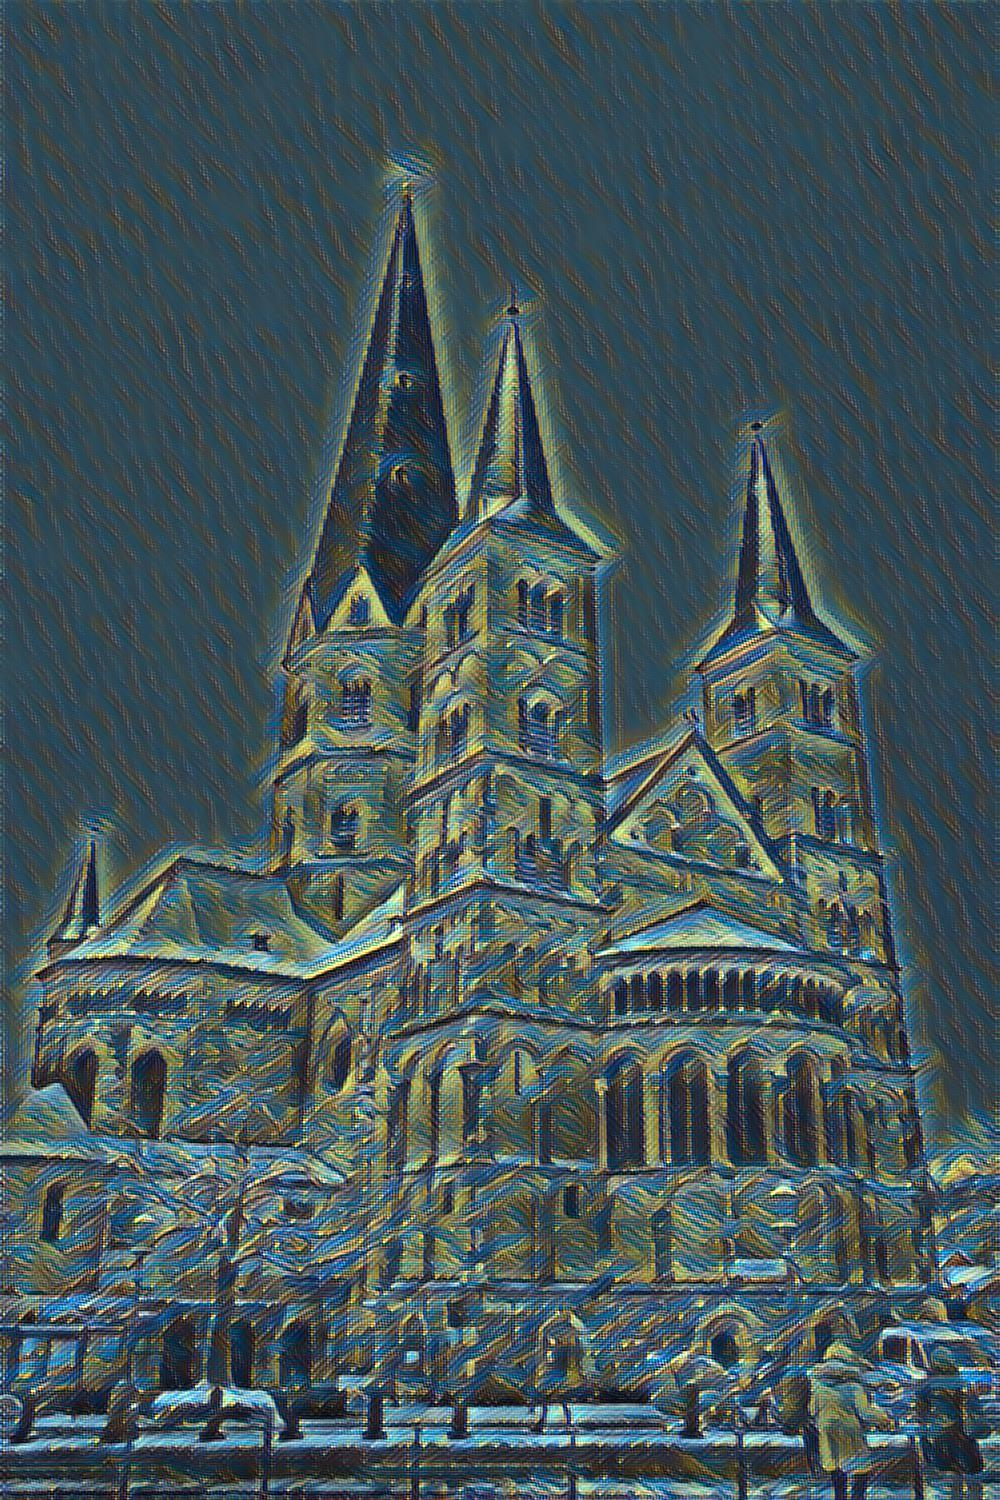
\includegraphics[width=0.495\textwidth, height=0.7\textheight]{bonn_muenster_starry_style_upper}
            \caption{\label{fig:clutter}Lower layers vs upper layers}
        \end{figure}

    \end{frame}

    \begin{frame}{Learning curve}

        \begin{figure}
            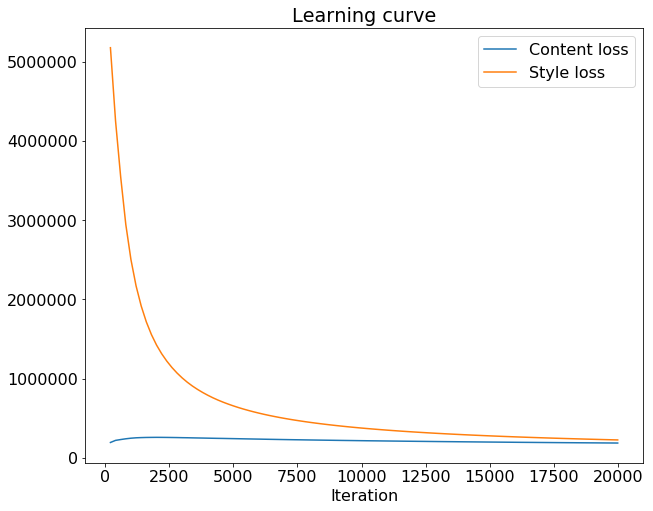
\includegraphics[width=\textwidth]{learningcurve}
        \end{figure}

    \end{frame}

    \begin{frame}{Stylization progression: iter 100}

        \begin{figure}
            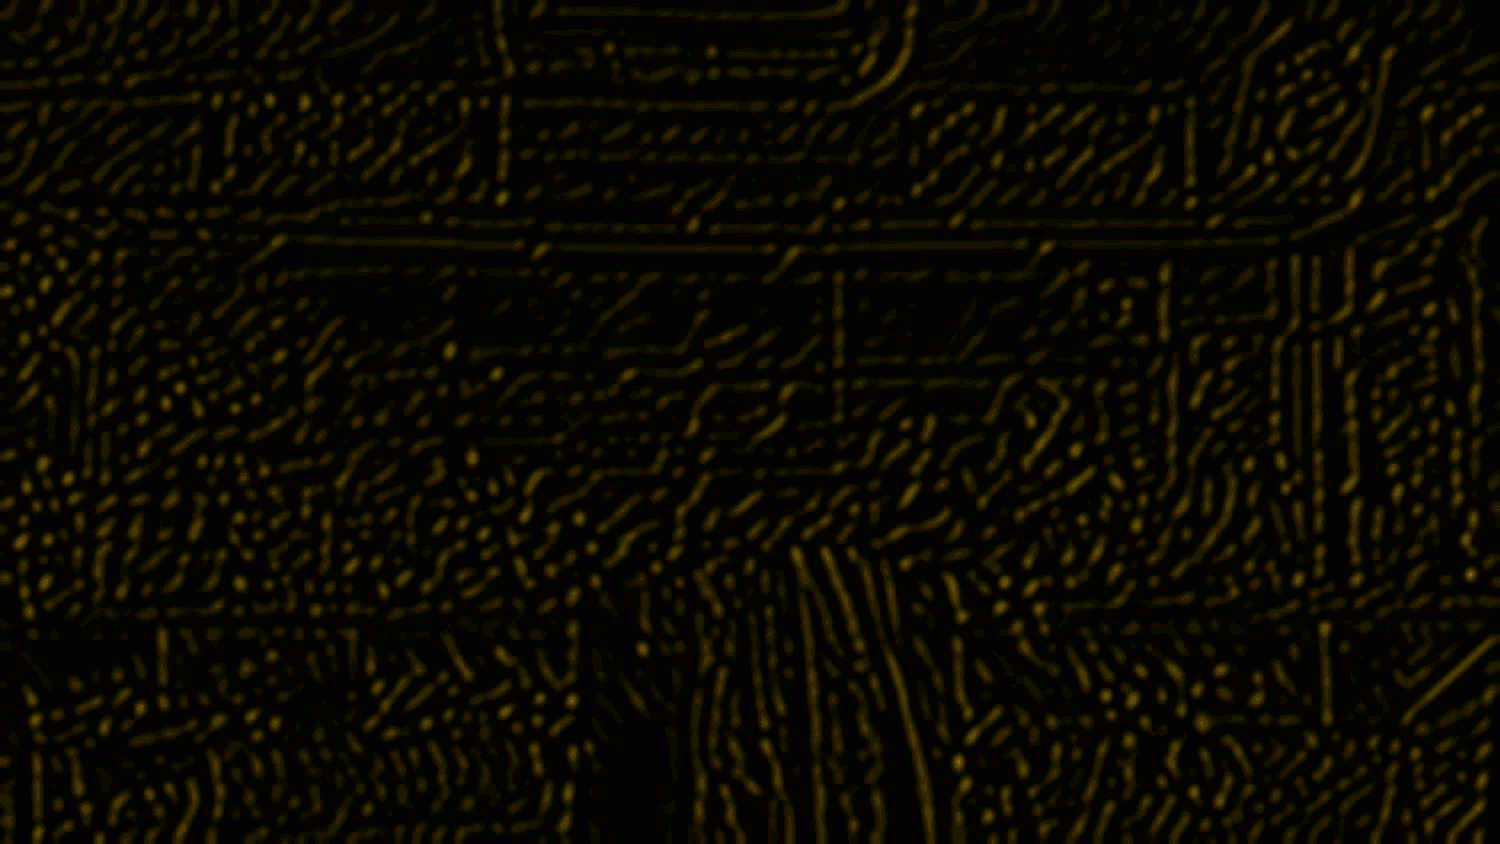
\includegraphics[width=\textwidth]{progression-0}
        \end{figure}

    \end{frame}

    \begin{frame}{Stylization progression: iter 500}

        \begin{figure}
            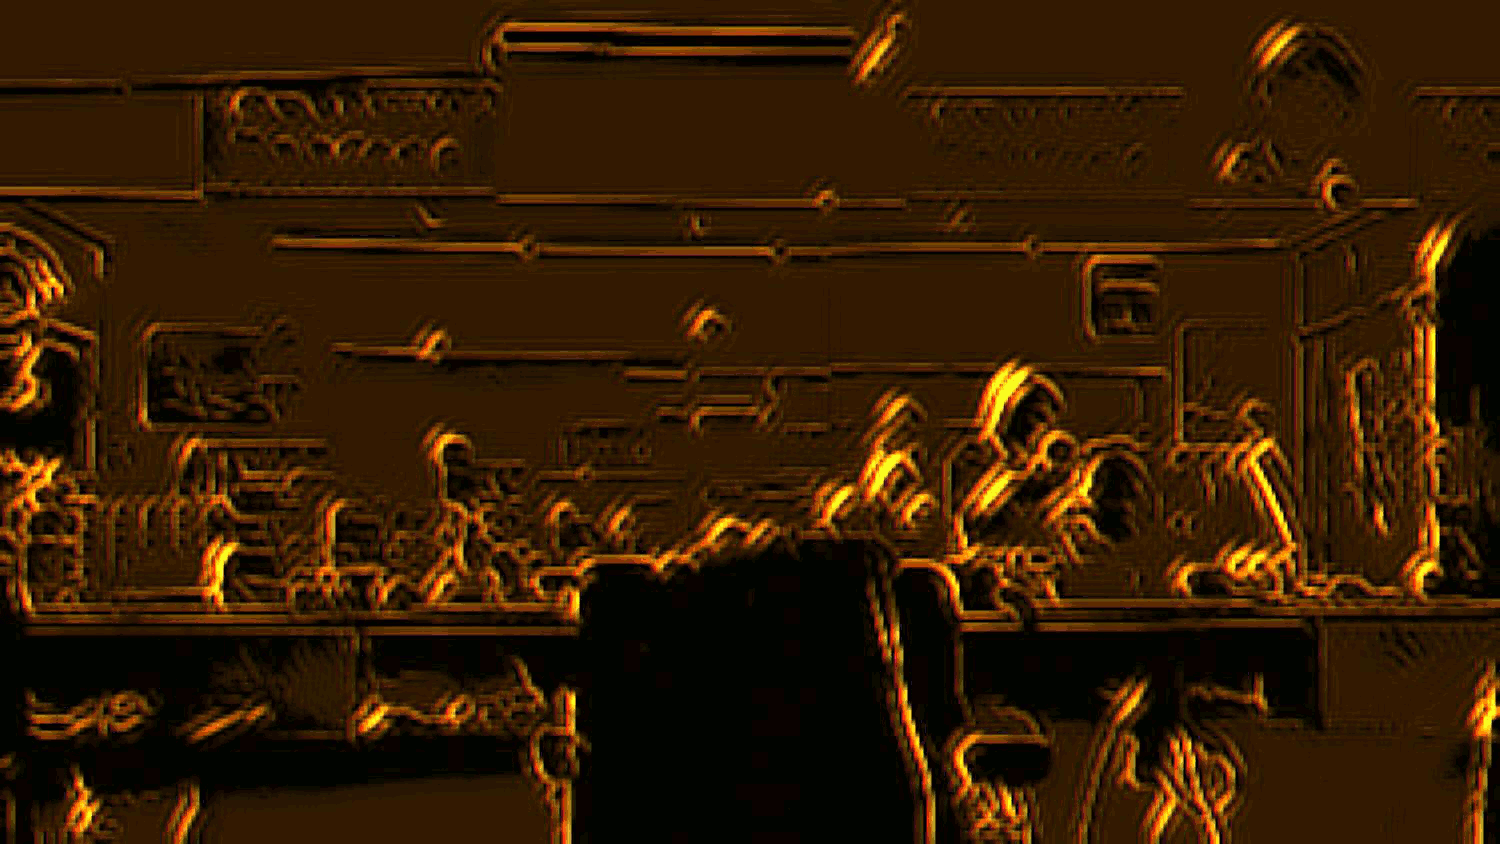
\includegraphics[width=\textwidth]{progression-1}
        \end{figure}

    \end{frame}

    \begin{frame}{Stylization progression: iter 1000}

        \begin{figure}
            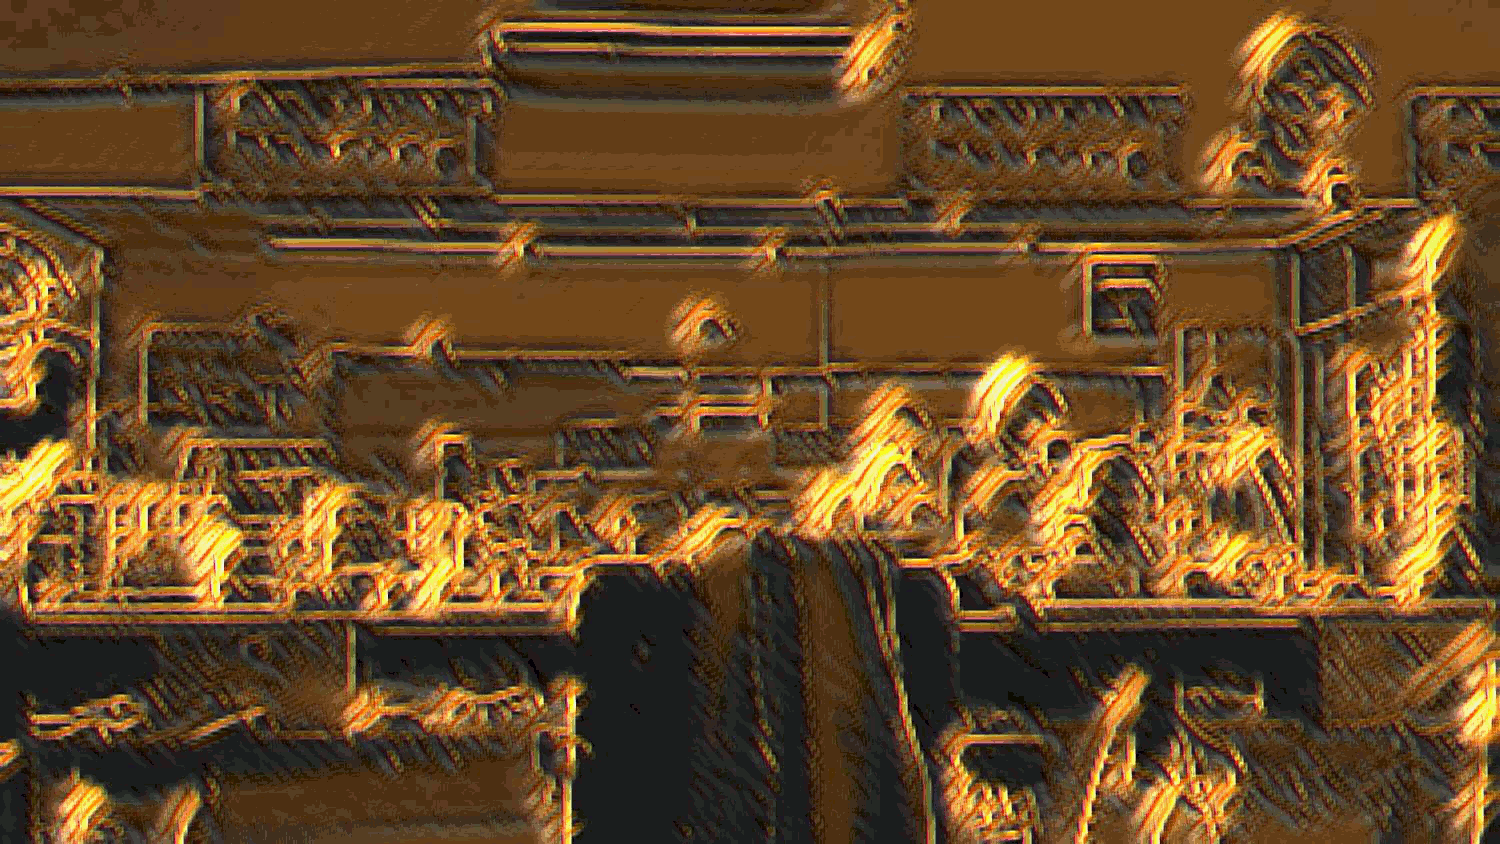
\includegraphics[width=\textwidth]{progression-2}
        \end{figure}

    \end{frame}

    \begin{frame}{Stylization progression: iter 5000}

        \begin{figure}
            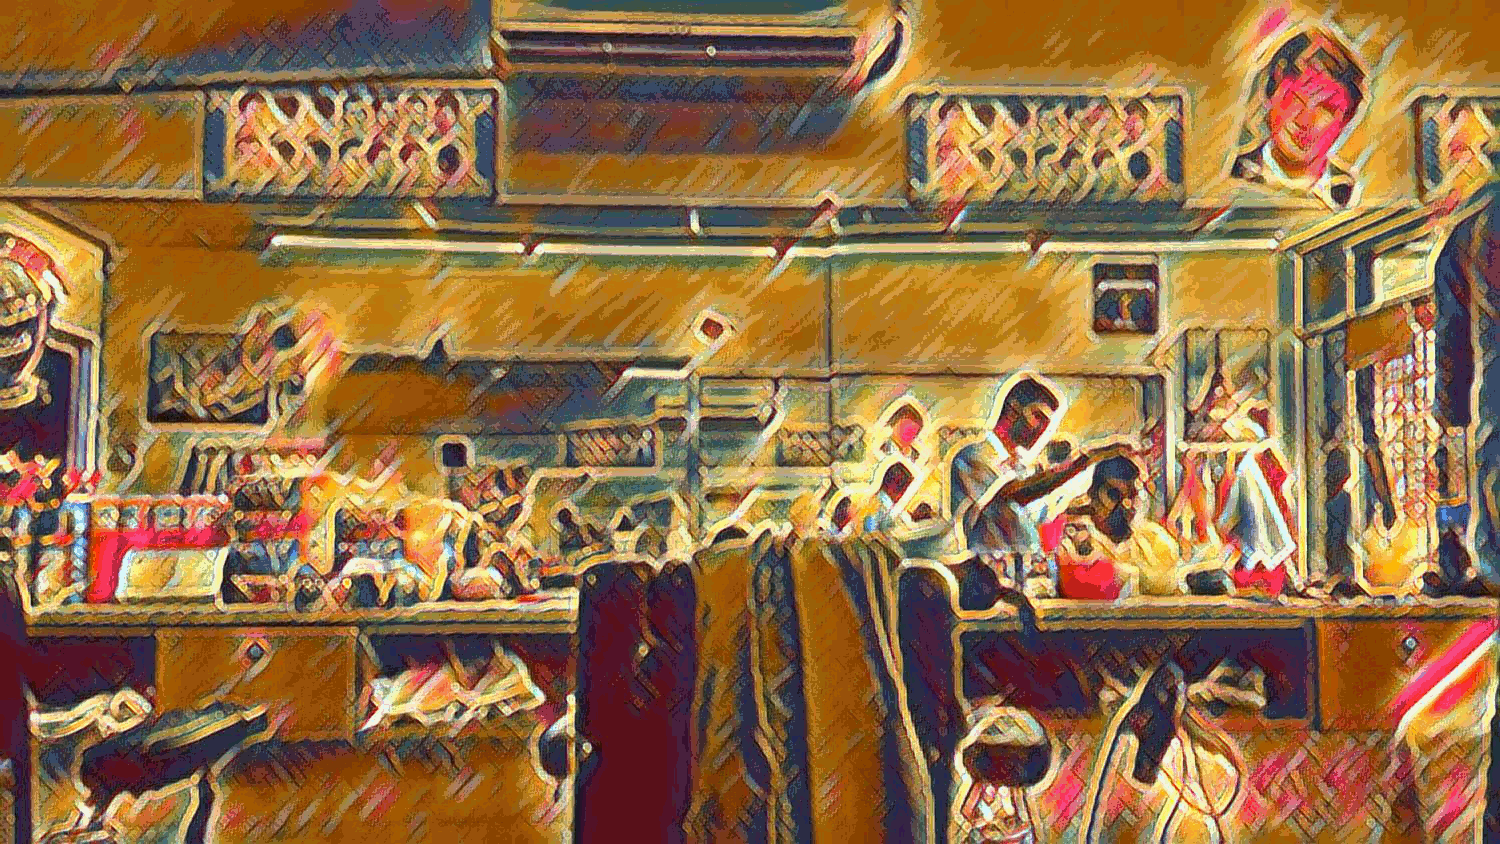
\includegraphics[width=\textwidth]{progression-3}
        \end{figure}

    \end{frame}

    \begin{frame}{Stylization progression: iter 10000}

        \begin{figure}
            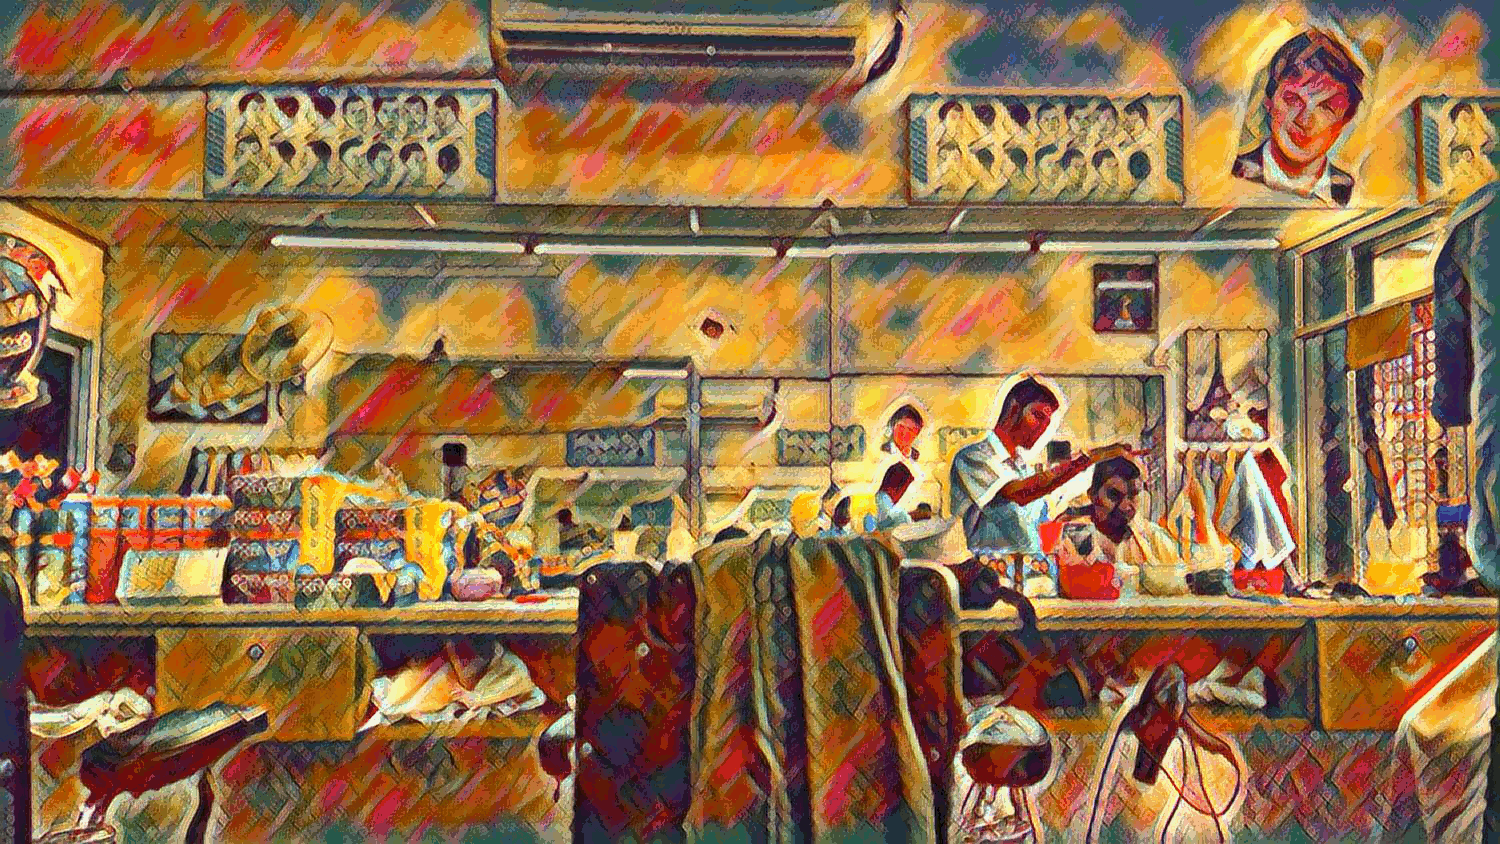
\includegraphics[width=\textwidth]{progression-4}
        \end{figure}

    \end{frame}

    \begin{frame}{Stylization progression: iter 20000}

        \begin{figure}
            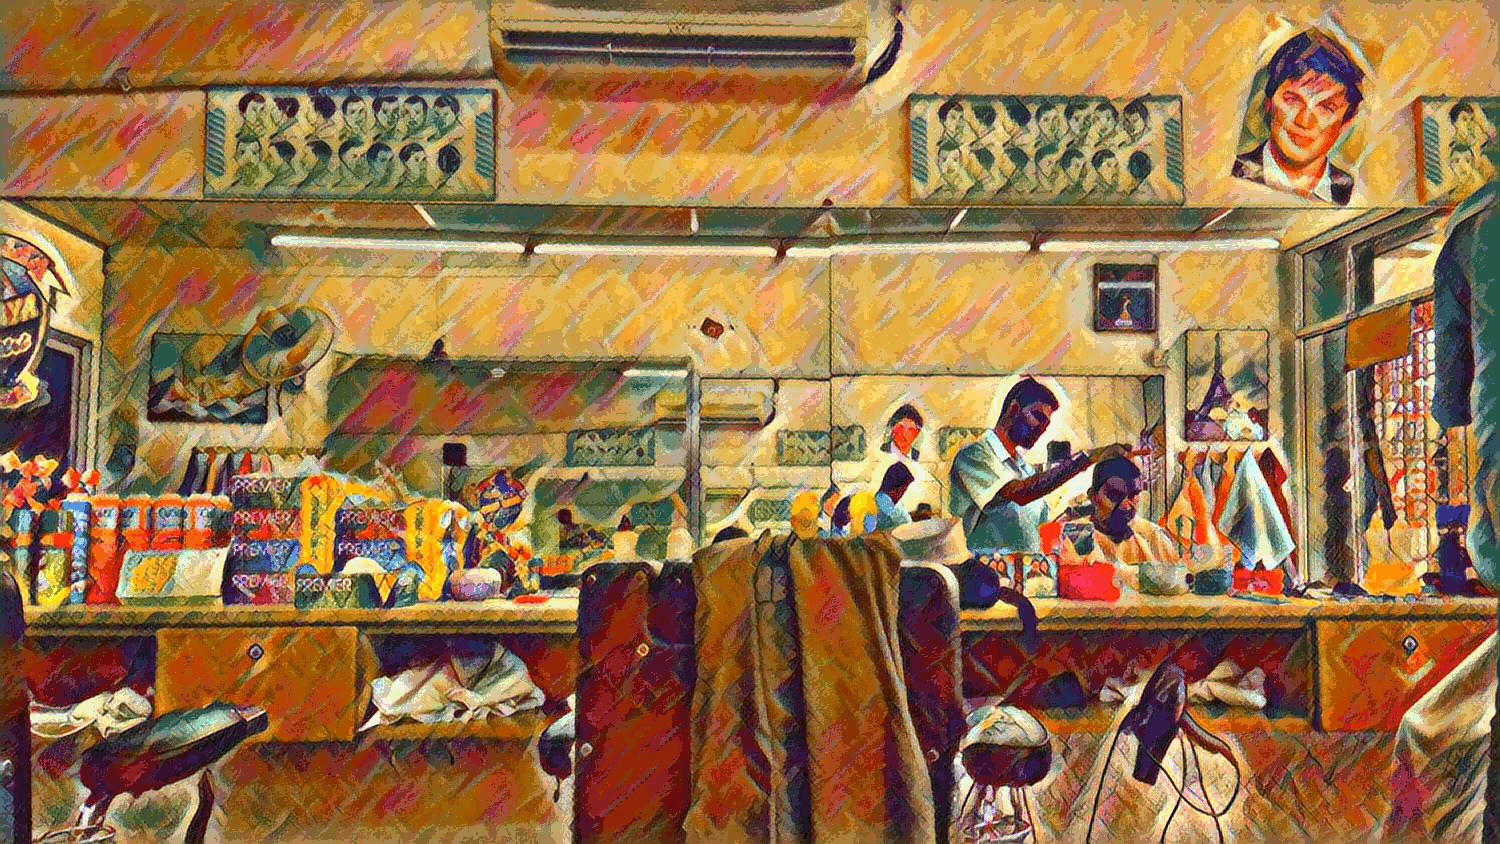
\includegraphics[width=\textwidth]{progression-5}
        \end{figure}

    \end{frame}

    \section{Conclusion}

    \begin{frame}{Conclusion}
        \begin{itemize}
            \item Johnson 2016 architecture is fast.
            \item InstanceNorm is a must.
            \item Careful tuning needed for different styles.
        \end{itemize}
    \end{frame}

    \begin{frame}{References}

        \begin{itemize}
            \item Gatys, Leon A., Alexander S. Ecker, and Matthias Bethge. "A neural algorithm of artistic style." arXiv preprint arXiv:1508.06576 (2015).
            \item Johnson, Justin, Alexandre Alahi, and Li Fei-Fei. "Perceptual losses for real-time style transfer and super-resolution." European Conference on Computer Vision. Springer International Publishing, 2016.
            \item Ulyanov, Dmitry, Andrea Vedaldi, and Victor Lempitsky. "Instance normalization: The missing ingredient for fast stylization." arXiv preprint arXiv:1607.08022 (2016).
        \end{itemize}
    \end{frame}

\end{document}
